% ****** Start of file apssamp.tex ******
%
%   This file is part of the APS files in the REVTeX 4.2 distribution.
%   Version 4.2a of REVTeX, December 2014
%
%   Copyright (c) 2014 The American Physical Society.
%
%   See the REVTeX 4 README file for restrictions and more information.
%
% TeX'ing this file requires that you have AMS-LaTeX 2.0 installed
% as well as the rest of the prerequisites for REVTeX 4.2
%
% See the REVTeX 4 README file
% It also requires running BibTeX. The commands are as follows:
%
%  1)  latex apssamp.tex
%  2)  bibtex apssamp
%  3)  latex apssamp.tex
%  4)  latex apssamp.tex
%
\documentclass[%
  reprint,
  superscriptaddress,
%groupedaddress,
%unsortedaddress,
%runinaddress,
%frontmatterverbose,
%preprint,
%preprintnumbers,
%nofootinbib,
%nobibnotes,
%bibnotes,
  amsmath,amssymb,
  aps,
  prapplied,
%pra,
%prb,
%rmp,
%prstab,
%prstper,
  floatfix,
]{revtex4-2}

\usepackage{graphicx}% Include figure files
\usepackage{dcolumn}% Align table columns on decimal point
\usepackage{bm}% bold math
\usepackage{hyperref}% add hypertext capabilities
\hypersetup{
  colorlinks=true, % Set 'true' to enable colored links
  linkcolor=black, % Color of internal links (sections, pages, etc.)
  citecolor=black, % Color of citations
  filecolor=black, % Color of file links
  urlcolor=black, % Color of URL links
}
\usepackage{svg}
\usepackage{epstopdf}
\usepackage[utf8]{inputenc}
\usepackage[T1]{fontenc}
\usepackage{amsmath}
\usepackage{amsfonts}
\usepackage{amssymb}
%\usepackage[mathlines]{lineno}% Enable numbering of text and display math
%\linenumbers\relax % Commence numbering lines

%\usepackage[showframe,%Uncomment any one of the following lines to test
%%scale=0.7, marginratio={1:1, 2:3}, ignoreall,% default settings
%%text={7in,10in},centering,
%%margin=1.5in,
%%total={6.5in,8.75in}, top=1.2in, left=0.9in, includefoot,
%%height=10in,a5paper,hmargin={3cm,0.8in},
%]{geometry}
\usepackage{subcaption}
\usepackage{hyperref}
\usepackage{siunitx}
\usepackage{mhchem}

%Define custom units for siunitx package
\DeclareSIUnit{\sample}{Sa}
\DeclareSIUnit{\octave}{Oct}
\DeclareSIUnit{\dBm}{dBm}

\begin{document}

\preprint{APS/123-QED}

\title{A coherently stimulated Brillouin spectrometer}

\author{Joel N. Johnson}
  \email{joel.johnson@nau.edu}
  \affiliation{Department of Applied Physics and Materials Science, Northern Arizona University, Flagstaff, AZ, 86011, USA}
  \affiliation{Center for Materials Interfaces in Research and Applications, Northern Arizona University, Flagstaff, AZ, 86011, USA}

\author{Co Authors}
  \affiliation{Department, Address}

\author{Ryan O. Behunin}
  \email{ryan.behunin@nau.edu}
  \affiliation{Department of Applied Physics and Materials Science, Northern Arizona University, Flagstaff, AZ, 86011, USA}
  \affiliation{Center for Materials Interfaces in Research and Applications, Northern Arizona University, Flagstaff, AZ, 86011, USA}

\date{\today}

\begin{abstract}
We present a novel coherently stimulated Brillouin spectrometer utilizing a detuned pump-probe design that exploits a relaxation of phase-matching requirements at small lengths, enabling room-temperature traveling-wave phonon spectroscopy at the micrometer scale with sub-\SI{10}{\femto\watt} sensitivity. This approach overcomes the limitations of traditional stimulated Brillouin techniques, particularly regarding phase-matching constraints and spatial resolution. We validated our instrument’s sensitivity with \SI{1}{\centi\meter} of UHNA3 fiber and \SI{100}{\micro\meter} of bulk carbon disulfide liquid, demonstrating its capability to measure Brillouin scattering in materials with low Brillouin gain or, with particular advantage, small effective lengths. This advancement opens new possibilities for nanometer-scale Brillouin spectroscopy and the development of nano-acousto-optic devices.

%\begin{description}
%\item[Usage]
%Secondary publications and information retrieval purposes.
%\item[Structure]
%You may use the \texttt{description} environment to structure your abstract;
%use the optional argument of the \verb+\item+ command to give the category of each item.
%\end{description}
\end{abstract}

\keywords{Brillouin scattering, phonon spectrometer, phase-matching relaxation, nanometer-scale spectroscopy, photonics, femtowatt, pump-probe, instrument, room-temperature, nano-acousto-optic devices}%Use showkeys class option if keyword display desired

\maketitle

%\tableofcontents


\section{Introduction}
\label{sec:Introduction}

Brillouin scattering, the inelastic interaction between light and acoustic phonons, is a fundamental phenomenon for probing the mechanical and structural properties of materials at microscopic scales. In spontaneous Brillouin scattering, thermally excited acoustic phonons scatter incident light, causing frequency shifts that reveal information about the material’s elastic properties and acoustic modes \cite{boyd2020nonlinear}. However, the weak signal inherent to spontaneous Brillouin scattering often demands long acquisition times and limits spatial resolution, posing challenges for high‐resolution material characterization.

Stimulated Brillouin scattering (SBS) uses intense optical fields to amplify the acoustic wave through a nonlinear optical process \cite{chiao1964stimulated}. In SBS, a strong pump laser interacts with a counter‐propagating Stokes wave in the medium, generating acoustic phonons via electrostriction. As the phonon population grows, it further amplifies the Stokes wave. In turn, that amplified Stokes wave interferes with the pump and reinforces the acoustic field, creating a positive feedback loop that drives exponential amplification. This mechanism enables more efficient excitation and detection of acoustic phonons and underpins numerous applications in optical signal processing, sensing, and high‐resolution spectroscopy including mechanobiology \cite{eggleton2013inducing, fotiadi2023brillouin, kobyakov2009stimulated, ippen1972stimulated, speziale2014brillouin, palombo2019brillouin, dil1982brillouin, eggleton2019brillouin, prevedel2019brillouin, conrad2019mechanical}.

%this whole paragraph needs to be rewritten to set up the phase matching restricitons that continue to pose a challenge\cite{yu2024chip} as a thing that our method solves.s
However, conventional SBS techniques struggle with short samples or materials of inherently low Brillouin gain \cite{rakich2012giant, gyger2020observation}. Because the Stokes amplitude depends on the product of the Brillouin gain coefficient, pump power, and interaction length, small volumes often yield weak signals unless extremely high optical powers are used. Moreover, while backward SBS sends the scattered wave in the opposite direction of the pump, parasitic reflections and pump leakage can still obscure the Stokes signal, demanding careful optical isolation and sometimes elaborate filtering. These constraints make it difficult to measure micro‐ and nanoscale devices, particularly if high optical intensities risk damaging sensitive samples. As a result, standard SBS approaches are not easily adapted to sub‐centimeter lengths or low‐gain media, prompting the need for new methods that maintain high sensitivity in short interaction regions.

To overcome these challenges, researchers have explored various approaches \cite{shin2013tailorable, van2015interaction, kittlaus2016large, djadaojee2020stimulated, gusev2018advances, gerakis2011coherent}. Techniques based on optical cavities increase the effective interaction length, but require precise alignment and are sensitive to environmental fluctuations \cite{pant2011cavity}. Forward Brillouin scattering methods, such as those demonstrated by Kittlaus et al. \cite{kittlaus2017chip}, offer relaxed phase‐matching conditions but introduce increased modal complexity. Meanwhile, coherent probe beam amplification can boost sensitivity, yet it can introduce additional noise and complexity because phase noise in laser sources can cause significant gain fluctuations \cite{shlomovits2015effect}.

Here, we demonstrate a detuned pump–probe design that relaxes the usual phase‐matching constraints at short lengths. This approach offers a new route to measure traveling‐wave phonons in sub‐centimeter or even micrometer‐scale samples at room temperature with unprecedented sensitivity. We demonstrate the capabilities of our instrument by measuring Brillouin scattering in \SI{1}{\centi\meter} of ultrahigh numerical aperture (UHNA3) fiber and \SI{100}{\micro\meter} of bulk carbon disulfide (\ce{CS2}) liquid. These measurements highlight the instrument’s ability to characterize materials with low Brillouin gain or small effective lengths.

The development of this coherently stimulated Brillouin spectrometer opens new avenues for nanometer‐scale Brillouin spectroscopy and advances the characterization and design of nano‐acousto‐optic devices. It holds promise for pushing research in material science, photonics, and sensing technologies toward higher spatial resolution and sensitivity, marking a significant step toward practical, room‐temperature Brillouin‐based spectroscopy and sensing solutions.

\section{Theoretical Framework}
\label{Theoretical Framework}

\subsection*{Coherently stimulated four-wave Brillouin scattering}
\label{Theoretical Framework:Coherently stimulated five-wave Brillouin scattering}
Traditional SBS, illustrated by the schematic in Fig.~\ref{fig:4-Wave-Brillouin-Scattering}(a) for the Stokes process, is a three-wave mixing process in which incident pump laser light of frequency \(\omega_{\mathrm{Pump}}\) inelastically scatters from a traveling-wave phonon of frequency \(\Omega\) to produce light that is frequency-shifted by the phonon frequency. In the Stokes process the phonon is retreating from the incident laser light and the scattered light is shifted down in frequency (\(\omega_{\mathrm{Stokes}} = \omega_{\mathrm{Pump}} - \Omega\)). Spatial overlap of the backscattered light with the incident laser light allows for interference of the two optical fields to produce a frequency at the difference of the two (\(\omega_{\mathrm{Pump}} - \omega_{\mathrm{Stokes}}\)). Since this difference frequency is exactly equal to the frequency of the acoustic field \(\Omega\), the beating of the incident pump light with the backscattered Stokes light produces an electrostrictive reinforcement of the acoustic wave. This driving of the acoustic wave in turn increases the scattering rate of the incident pump light, producing a positive feedback process and an exponential increase of the amplitude of the backscattered Stokes wave.

\begin{figure*}[t]
  \centering
  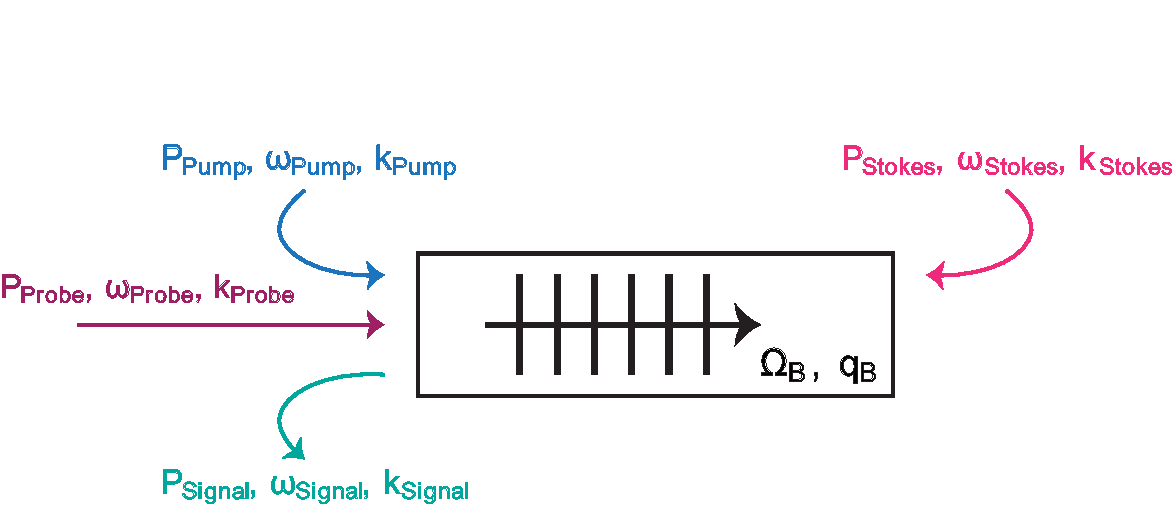
\includegraphics[width=.5\textwidth]{4-Wave-Brillouin-Scattering.pdf}
  \caption{Illustration of 4-Wave Brillouin Scattering.}
  \label{fig:4-Wave-Brillouin-Scattering}
\end{figure*}

Fig.~\ref{fig:4-Wave-Brillouin-Scattering}(b) illustrates coherently stimulated four-wave Brillouin scattering for the Stokes process. We introduce a strong, controlled external Stokes wave of frequency \(\omega_{\mathrm{Stokes}}\) that drives electrostrictive reinforcement of the acoustic field in the medium. The backscattered Stokes light is normally collected in an SBS process, but the external Stokes laser overwhelms it. To resolve this, we inject light of a distinct frequency \(\omega_{\mathrm{Probe}}\) from an additional external laser which copropagates with the Pump and backscatters in the medium from the strongly driven acoustic field. This produces backscattered Signal light to be collected (\(\omega_{\mathrm{Signal}} = \omega_{\mathrm{Probe}} - \Omega\)) which is spectrally distinct from the high-powered Stokes laser light.

To describe this interaction and characterize the performance of the instrument, we derive the coupled-wave equations for the four-wave mixing process in Appendix~\ref{Appendix:Coupled-Wave Equations}. These equations describe the relationship between the optical fields and the acoustic field in the material and result in the following expression for the scattered power of the backscattered signal,
\\
\begin{equation}
  P_{Sig} = \frac{1}{4}(G_{B}L)^{2}P_{P}P_{S}P_{Pr}sinc^{2}\left(\frac{\Delta kL}{2}\right),
  \label{Eq:Theoretical Framework:Scattered Power} %compress sinc term into Psi here?
\end{equation}
\\
where \(P_P\), \(P_S\), and \(P_Pr\) are the powers of the pump, Stokes, and probe lasers, respectively. \(G_B\) is the effective Brillouin gain, given by
\\
\begin{equation}
  G_{B} = \frac{g_{0}}{A_{eff}}\frac{\left(\frac{\Gamma_{B}}{2}\right)^{2}}{(\Omega - \Omega_{B})^{2} + \left(\frac{\Gamma_{B}}{2}\right)^{2}},
  \label{Eq:Effective Brillouin Gain}
\end{equation}
\\
with the on-resonance gain factor of the material given by
\\
\begin{equation}
  g_{0} = \frac{\gamma_{e}^{2}\omega^{2}}{nvc^{3}\rho_{0}\Gamma_{B}}.
\end{equation}
\\
Here, \(\gamma_e\) is the electrostrictive constant, \(\omega\) is the pump frequency, \(n\) is the refractive index of the material, \(v\) is the sound speed of the material, \(c\) is the speed of light, \(\rho_0\) is the mean density of the material, and \(\Gamma_B\) is the Brillouin linewidth, or phonon dissipation rate, of the material. In Eq.~\ref{Eq:Effective Brillouin Gain}, \(\Omega_B\) is the resonant Brillouin frequency of the material, \(A_{Eff}\) is the effective area of the material, \(\Delta k\) is the wavevector mismatch between the optical fields, to be discussed next, and \(L\) is the effective length of the material.


\subsection*{Phase matching relaxation}
\label{Theoretical Framework: Phase matching relaxation}
In all nonlinear optical processes, efficiency is maximized when phase matching conditions are satisfied. A frequency mismatch (energy unconservation) or a wavevector mismatch (momentum unconservation) each result in drastically reduced efficiency of a given process.\cite{maker1962effects} This can be seen by Eq.~\ref{Eq:Theoretical Framework:Scattered Power}, where the wavevector mismatch, \(\Delta k\), is contained within a \(\mathrm{sinc^2}\) function. This \(\mathrm{sinc^2}\) term thereby defines the phase matching bandwidth of the system, notably scaling with effective interaction length \(L\).

We apply this wavevector mismatch allowance to the pump and probe waves (\(\Delta k = k_{\mathrm{Pump}} - k_{\mathrm{Probe}}\)) so that the backscattered signal is different than the applied Stokes wave. This choice allows for selection of the signal and rejection of the Stokes with a bandpass filter. Expressed in terms of wavelengths, this gives
\\
\begin{equation}
  \Delta k = \frac{4\pi n\Delta\lambda}{\lambda_{Pump}\lambda_{Probe}} \approx \frac{4\pi n\Delta\lambda}{\lambda_{Pump}^{2}}.
\end{equation}
\\
We can apply this to the phasematching bandwidth term to find the fraction of maximum scattered power, \(\Phi\), that can be expected for a given interaction length, \(L\), and phase mismatch \(\Delta\lambda\) between the pump and probe,
\\
\begin{equation}
  \Phi \equiv sinc^{2}\left(\frac{2\pi n\Delta\lambda L}{\lambda_{Pump}^{2}}\right).
  \label{Eq:Phi}
\end{equation}
\\
Using this expression for \(\Phi\), we see that for an effective length of \SI{1}{\meter}, a wavelength mismatch of only \SI{0.6}{\pico\meter} from a typical wavelength of \SI{1.55}{\micro\meter} pump light in UHNA3 fiber drops the scattered power to half of the maximum. However, for shorter effective lengths the wavevector mismatch becomes more forgiving; a \SI{36}{\pico\meter} mismatch preserves 82.5\% of the maximum signal for a length of \SI{1}{\centi\meter} under identical conditions. This separation translates to about \SI{4.5}{\giga\hertz}, providing enough spectral separation for the backscattered signal to be isolated from the applied Stokes light.

Furthermore, for decreasing lengths, Eq.~\ref{Eq:Phi} predicts an increase in the fraction of maximum signal produced, given equivalent pump--probe detuning, as the \(\mathrm{sinc^2}\) function is sampled closer to its peak center. Alternatively, as length decreases, the probe may be further detuned from the pump and still achieve the same fraction of the maximum signal as for longer lengths, perhaps offering a slight advantage in noise reduction. It should be noted that the scattered power, as given by Eq.~\ref{Eq:Theoretical Framework:Scattered Power}, scales with the square of the effective length. Thus, while smaller lengths allow for the ability to capture a larger fraction of this maximum scattered power, the actual amount of scattered power decreases dramatically as length decreases.

\section{Methods}\label{Methods}
\subsection*{Instrument design}
\label{Methods:Instrument Design}

\begin{figure*}[htbp]
\centering
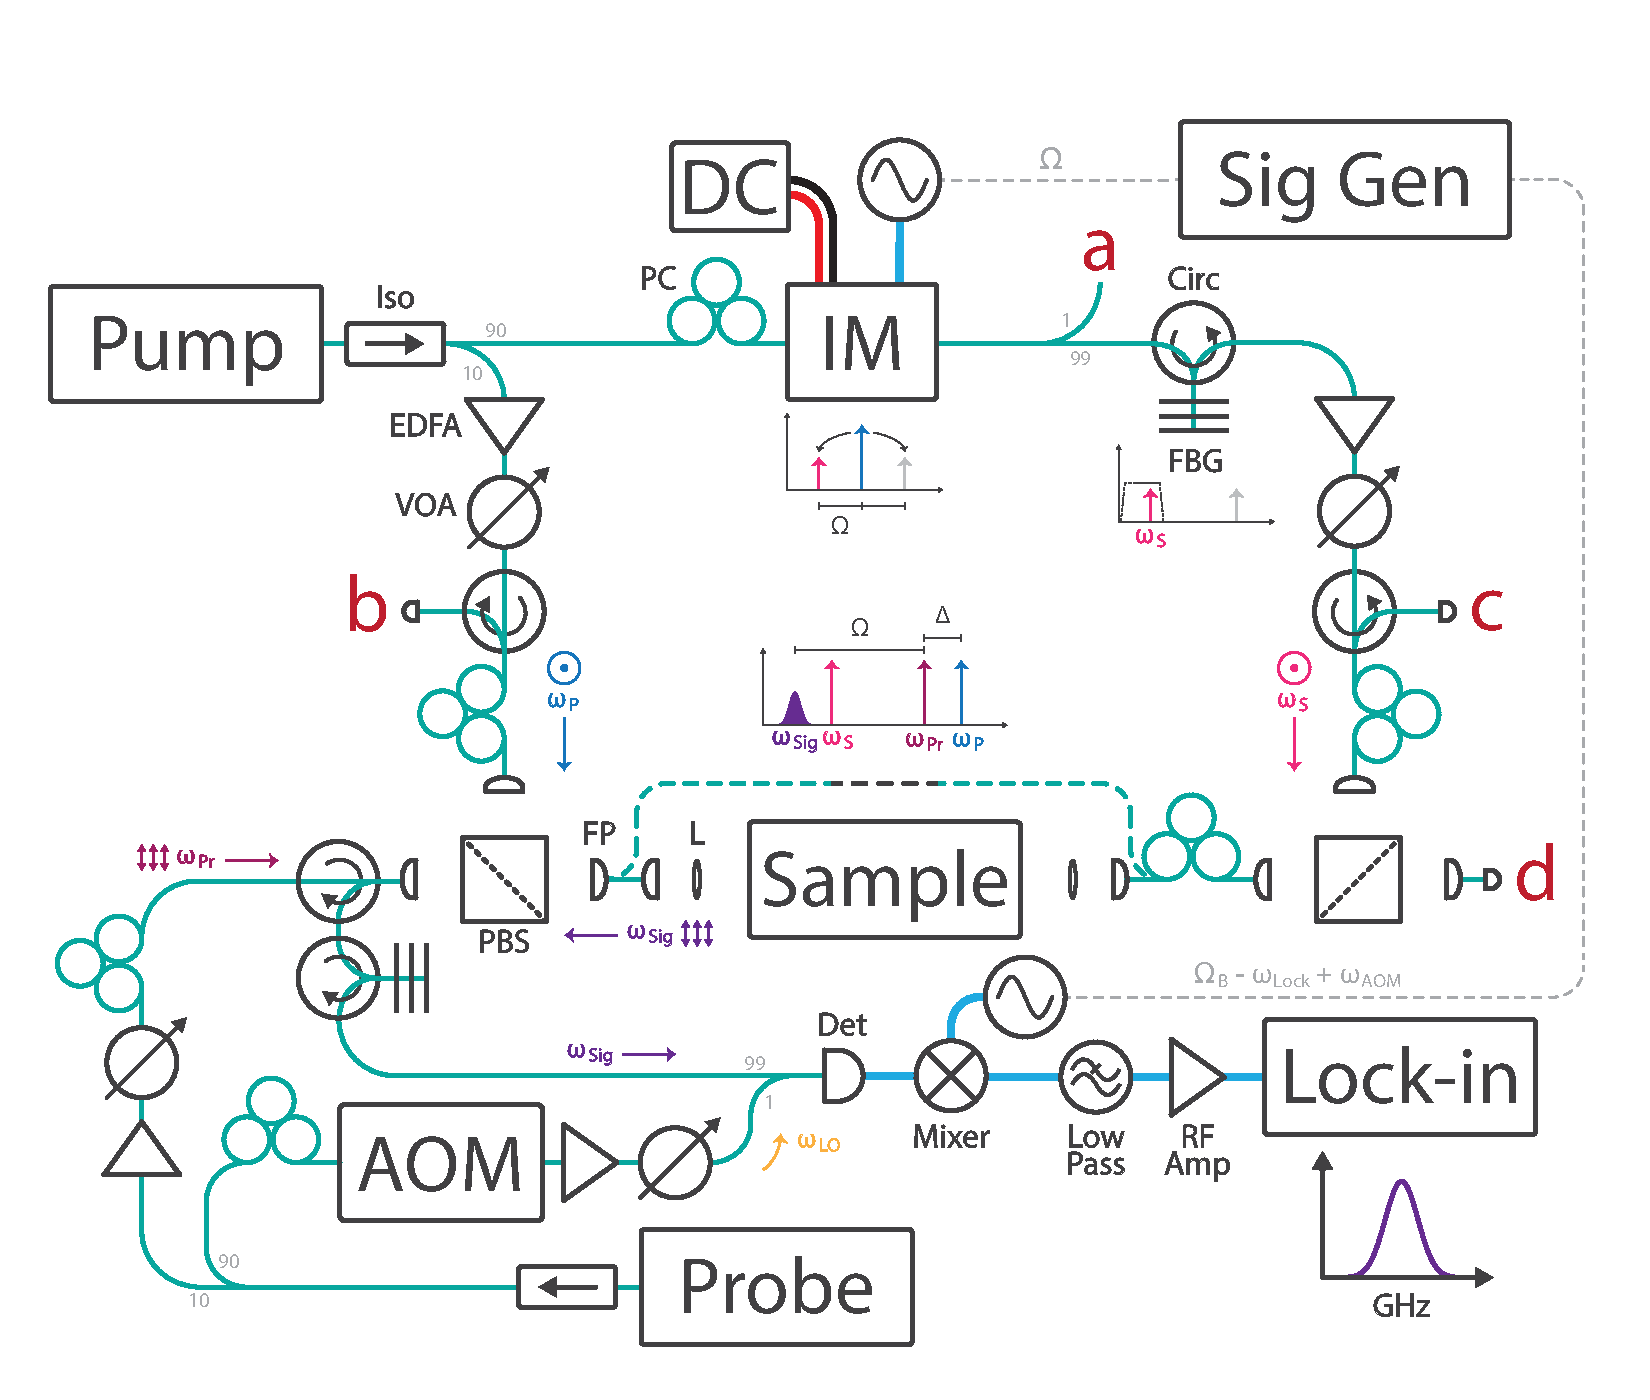
\includegraphics[width=\textwidth]{Instrument-Design-V1.pdf}
\caption{
Design schematic of a coherently stimulated phonon spectrometer. A tunable continuous-wave (CW) laser at approximately \SI{1.55}{\micro\meter} emits light that passes through an isolator (Iso) and a splitter, diverting 10\% to a \SI{27}{\dBm} EDFA followed by a variable optical attenuator (VOA). This pump light (\(\omega_P\)) is polarization-controlled to reflect off a polarizing beam splitter (PBS) and is recoupled to fiber via a fiber port (FP), then directed to the sample either by direct fiber coupling or through a pair of FPs and lenses (L) for free-space samples. After passing through the sample, the pump light traverses a corrective polarization controller that mitigates fiber twists and bends before reflecting off a second PBS, where it is routed to port (c) for power monitoring. To synthesize the Stokes wave, a 90\% split from the original pump is processed through an intensity modulator (IM) and a fiber Bragg grating (FBG), generating a Stokes sideband downshifted from the pump by \(\Omega\). This frequency shift is swept via a signal generator to capture \(\Omega_B\). A 99/1 splitter provides a tap at port (a) to optimize Stokes synthesis. The Stokes wave (\(\omega_S\)), amplified by a \SI{1}{\watt} EDFA and VOA-controlled, counter-propagates along the pump path and is monitored at port (b). A second tunable CW laser, detuned from the pump, generates the probe wave (\(\omega_{Pr}\)), which is amplified by a \SI{1}{\watt} EDFA, attenuated variably, and polarization-controlled to pass through the initial PBS where it is incident on the sample. Backscattered signal light (\(\omega_{Sig}\)) transmits back through the PBS, while unscattered probe light transmits to a power meter at port (d). A circulator parts the signal from the probe path, with an FBG filtering out any unwanted noise or Stokes light. Finally, the signal is heterodyned with an EDFA-amplified, AOM-shifted local oscillator (LO) derived from the probe laser and directed to a photodiode for detection. The resulting RF signal is mixed with an AC LO supplied by the signal generator which sweeps synchronously with the Stokes synthesis frequency, and collected by a lock-in amplifier for data processing.
}
\label{fig:Instrument Design}
\end{figure*}

Figure~\ref{fig:Instrument Design} shows the instrument’s design. A pump and Stokes wave is synthesized from a single tunable laser source for coherent stimulation of a sample. The pump wave (\(\omega_{\mathrm{Pump}}\)) is amplified by an erbium-doped fiber amplifier (EDFA) and passed through a variable optical attenuator (VOA) for power control. The output is then polarization-controlled to reflect at a polarizing beam splitter (PBS) for injection into the sample. For Stokes synthesis, an AC signal (\(\Omega\)) is supplied to an intensity modulator (IM) with carrier frequency nulled and a tunable filter is used to select the lower-frequency Stokes side band (\(\omega_{\mathrm{Pump}} - \Omega\)). This Stokes light is then amplified by an EDFA, passed through a VOA, and polarization-controlled to reflect at a second PBS for couter-propagation to the pump through the sample.

A separate tunable laser is used to supply a probe wave (\(\omega_{\mathrm{Probe}} = \omega_{\mathrm{Pump}} + \Delta k\)) and local oscillator (LO). Probe light is amplified by an EDFA and passed through a VOA and a polarization controller aligns the polarization for transmission through the first PBS whereby it copropagates with the pump through the sample. Backscattered light exits the sample and transmits back through the first PBS, whereas the orthogonally polarized Stokes light reflects at this same point to be diverted to a tap for power monitoring. The backscattered signal (\(\omega_{\mathrm{Signal}} = \omega_{\mathrm{Probe}} - \Omega\)) then routes through two subsequent circulators for spectral filtering by a \SI{5}{\giga\hertz} bandpass tunable filter. This filter allows the desired backscattered signal to pass while rejecting any reflected probe light as well as any reflected, transmitted, or backscattered light from the pump or Stokes waves that was not already diverted by the PBS.

The filtered signal then heterodynes via a 99-1 splitter with the LO which is frequency-upshifted by an acousto-optic modulator (AOM) (\(\omega_{\mathrm{LO}} = \omega_{\mathrm{Probe}} + \omega_{\mathrm{AOM}}\)) and controlled to be copolarized with the signal. Of the resulting frequencies from the heterodyne process, only the difference frequency term is considered, as all others are beyond the range of detection. This heterodyned signal (\(\omega_{\mathrm{Signal}} = \Omega + \omega_{\mathrm{AOM}}\)) is then captured by a photodiode detector and heterodyned again by a radio frequency (RF) mixer with a second AC signal (\(\Omega + \omega_{\mathrm{AOM}} - \omega_{\mathrm{Lock}}\)), where \(\omega_{\mathrm{Lock}}\) is a fixed-frequency to be detected by a lock-in amplifier set to this frequency after being passed through a low-pass filter and amplified by an RF amplifier. Synchronous sweeping of both AC signals, each involving \(\Omega\), allows for \(\omega_{\mathrm{Lock}}\) to remain fixed throughout measurement over a frequency range.

\subsection*{Experimental Techniques}
\label{Methods:Experimental Techniques}
We optimized the signal-to-noise ratio (SNR) of our instrument through specific design choices and device settings. Our setup simultaneously generates pump, Stokes, and probe optical fields for coherently stimulated Brillouin scattering. The pump laser provides \(\sim\!\SI{45}{\milli\watt}\) total output, of which 10\% is split and amplified to \(\sim\!\SI{0.5}{\watt}\) for the pump field; the remaining 90\% is frequency-shifted and amplified to \(\sim\!\SI{1}{\watt}\) for the Stokes field. Likewise, the probe laser also outputs \(\sim\!\SI{45}{\milli\watt}\), with 10\% amplified to \(\sim\!\SI{1}{\watt}\) for the probe field and the remaining 90\% reserved for the local oscillator (LO). To combine the backscattered signal and LO with minimal loss, we use a 99/1 splitter instead of a typical 50/50, preserving 99\% of the signal. The LO is therefore amplified to \(\sim\!\SI{230}{\milli\watt}\) so the total optical power at the detector remains below the \(\SI{2.4}{\milli\watt}\) damage threshold. After detection, the electronic signal is mixed with a \SI{17}{\dBm} AC reference and further amplified by \SI{23}{\dBm} before input to the lock-in amplifier. We find that running both the pump and probe lasers in “whisper” mode (as opposed to “dither”) significantly enhances the measured SNR.

We use a Zurich Instruments HF2LI \SI{50}{\mega\hertz} lock-in amplifier whose demodulator settings are carefully tuned to maximize SNR. A \SI{10}{\mega\hertz} reference clock from the signal generator is fed into the lock-in to synchronize timing. The input-signal range, which sets the analog input amplifier’s gain, should exceed the measured signal (including any DC offset) by at least a factor of two. This is best achieved by using the lock-in software’s \emph{auto} feature, which continuously adjusts the range over a rolling \SI{100}{\milli\second} window. We set the input coupling to AC, insert a high-pass filter to remove DC components, and choose \(\SI{1}{\mega\ohm}\) input impedance. For noise suppression, we also engage the lock-in’s eighth-order low-pass filter (roll-off \SI{48}{\decibel\per\octave}) and sample the data at \(\SI{1.84}{\mega\sample\per\second}\), the maximum rate available.

Further SNR improvements are gained by narrowing the lock-in’s low-pass filter bandwidth to match both the sub-\si{\hertz} natural linewidth of the heterodyne signal and the thermally-driven frequency drift of the apparatus. After a \(\sim\!\SI{30}{\minute}\) warm-up, we observe less than \SI{100}{\hertz} of drift in the detected signal frequency, so we typically set a \SI{100}{\hertz} low-pass bandwidth for multi-hour measurements. For shorter scans (\(< \SI{15}{\minute}\)), we can reduce this bandwidth to \SI{40}{\hertz} if needed. In addition to linewidth variability, the signal’s center frequency can shift due to thermal changes in the AOM and related electronics. Although \(\Omega\) is nominally controlled to sub-hertz precision by the signal generator, our AOM’s shift \(\omega_{\mathrm{AOM}}\) drifts from \SI{40}{\mega\hertz} up to \(\sim\!\SI{40.00082}{\mega\hertz}\) over roughly \SI{30}{\minute}. Once at thermal equilibrium, the AOM remains stable within \(\pm\SI{50}{\hertz}\), enabling a reliable lock-in frequency reference and minimal filter bandwidth. This stability is crucial for repeatable, high-resolution Brillouin measurements.

\section{Results}\label{Results}
\subsection*{Instrument sensitivity}
\label{Results:Instrument sensitivity and SBS comparison}

\begin{figure}[t]
  \centering
  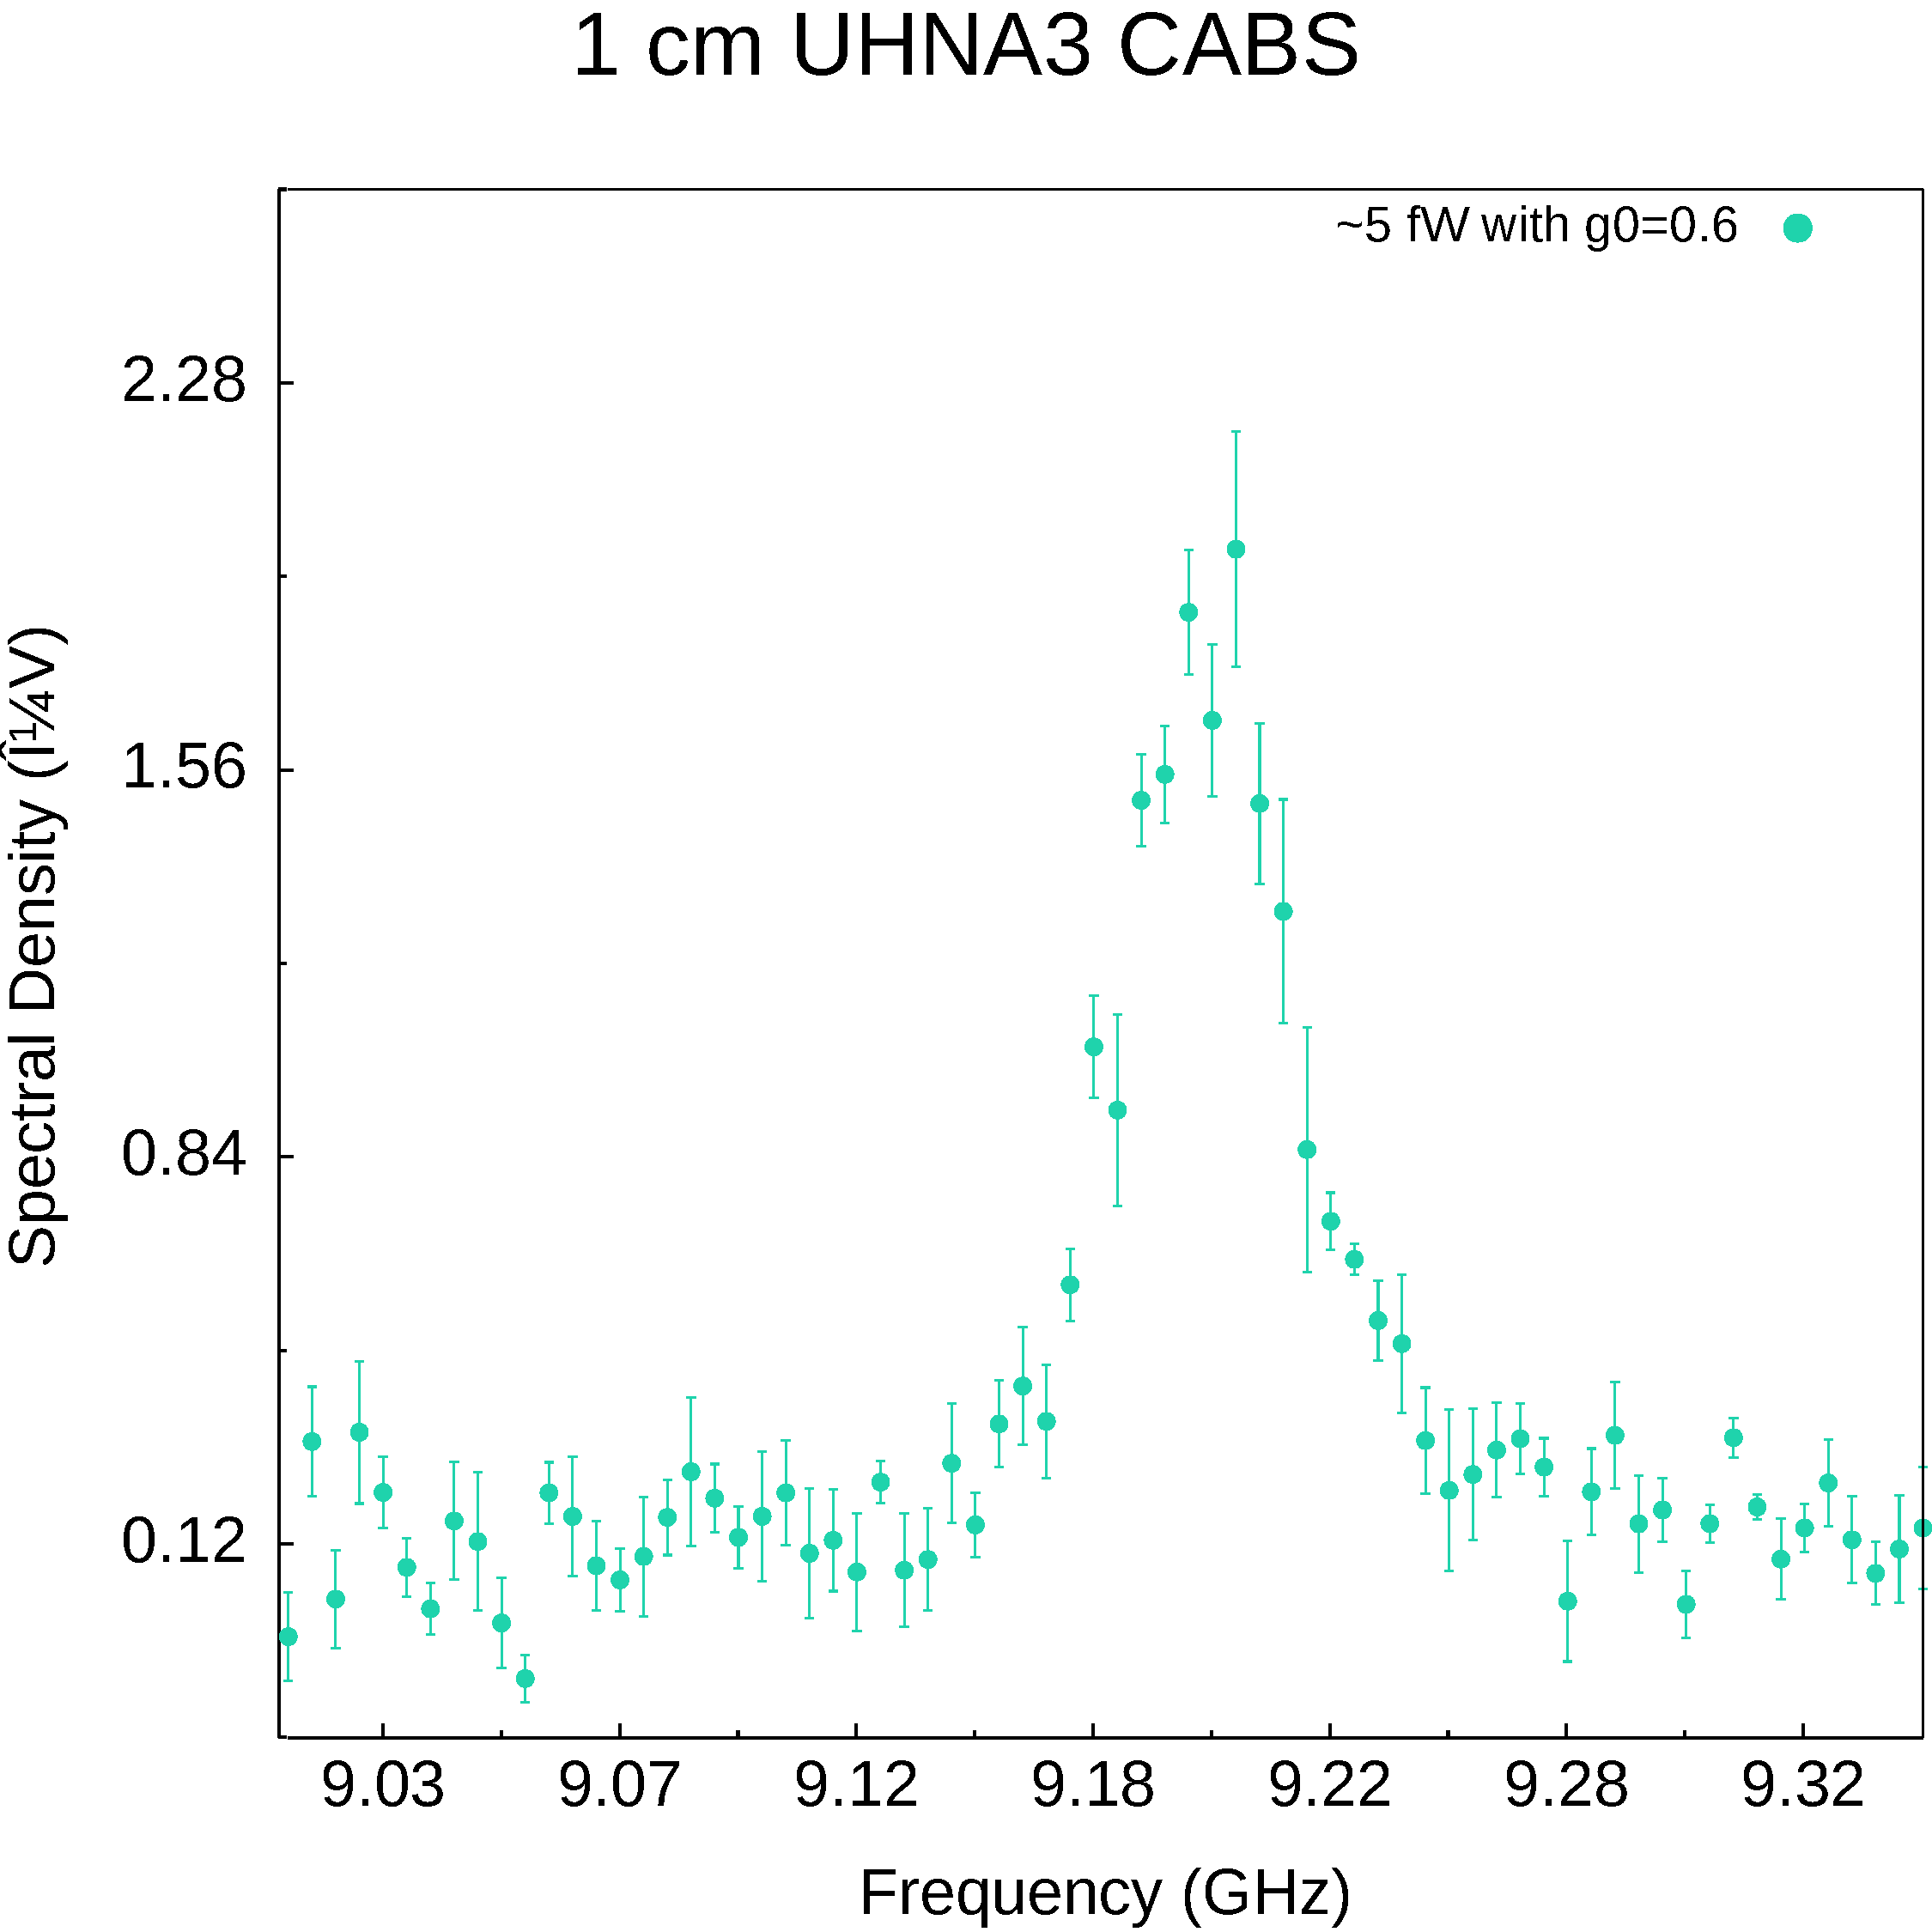
\includegraphics[width=.45\textwidth]{5fWSensitivity.pdf}
  \caption{\(\sim\SI{5}{\femto\watt}\) sensitivity measurement}
  \label{fig:5fWSensitivity}
\end{figure}

We begin by testing the sensitivity of the instrument as a way of defining a performance metric for the instrument which can be used to indicate what material, power, and length combinations might be possible to measure. From Eq.~\ref{Eq:Theoretical Framework:Scattered Power}, the sensitivity of the instrument is the minimum scattered power, \(P_{Sig}\), to produce a statistically significant measurement. To determine this, we target a specific length, \(L\), of a sample of known effective Brillouin gain, \(G_B\). We keep the pump-probe detuning, \(\Delta\lambda\), constant across measurements and record the pump, Stokes, and probe optical powers to calculate the scattered power. Starting with sufficient optical powers to produce a clearly distinguishable measurement, we gradually reduce the optical powers until the sensitivity floor is reached.

To serve as our sensitivity testbed, we prepared \SI{1}{\centi\meter} of Nufern's UHNA3 fiber, a well-studied fiber with known effective Brillouin gain\cite{behunin2015long}. Additionally, UHNA3 fiber offers several properties that make it ideal for this task of unambiguous detection of the Brillouin signal as it diminishes with each subsequent reduction in optical powers. First, it offers a Brillouin shift that is spectrally far from that of the single-mode fiber (SMF28) which constitutes much of the instrument. This ensures that the Brillouin response of the sample is not conflated with the Brillouin response of the instrument itself. Additionally, the core of UHNA3 fiber features a high concentration of germanium which improves the optical and acoustic guidance in the fiber as a result of the large refractive index difference between core and cladding. Finally, UHNA3 fiber offers a high optomechanical nonlinear response, with an effective Brillouin gain of \SI{0.6}{\per\watt\per\meter} measured at room temperature\cite{behunin2015long}. This gain factor is larger than that of SMF28 by an order of magnitude\cite{nikles1997brillouin}.

Figure~\ref{fig:5fWSensitivity} presents a measurement in which the instrument’s sensitivity reaches \(P_{Sig}\!= \SI{5}{\femto\watt}\). Each trace is the average of five consecutive scans, and an average of five background scans has been subtracted to isolate the signal. Error bars represent the standard error (\(1\sigma\) of the mean). By comparing the peak amplitude at resonance to the off-resonance baseline, we estimate an SNR greater than 5. Under a normal-noise assumption, an SNR of 5 corresponds to a \(5\sigma\) significance level (99.7\% confidence). Achieving this \SI{5}{\femto\watt} threshold demonstrates the feasibility of measuring weaker signals in materials with lower Brillouin gain or smaller effective lengths. Table~\ref{tab:sensitivity} in Appendix~\ref{} summarizes the relevant measurement parameters and on-resonance power calculations.

\begin{table}[h]
    \centering
    \begin{tabular}{|c|c|c|c|c|c|}
        \hline
        \(G_B\) & \(L\) & \(P_P\) & \(P_S\) & \(P_{Pr}\) & \(\Delta\lambda\) \\
        (\si{\per\watt\per\meter}) & (\si{\meter}) & (\si{\micro\watt}) & (\si{\micro\watt}) & (\si{\micro\watt}) & (\si{\pico\meter}) \\
        \hline
        0.6 & 0.01 & 506 & 504 & 2.01 & 20 \\
        \hline
    \end{tabular}
    \caption{Measurement parameters for sensitivity measurement and calculation.}
    \label{tab:sensitivity}
\end{table}

\subsection*{Measurements}
\label{Results:Measurements}

We demonstrate the capabilities of the instrument on two common sample classes: fiber and bulk material. For a fiber sample we again choose UHNA3 for its higher nonlinear response and excellent optical and acoustic guidance. In contrast to the sensitivity measurements, we now seek to demonstrate the full measuring capabilities of the instrument and so apply all available optical power (\(\sim\!\SI{1.5}{\watt}\)) to maximize the backscattered signal from the sample. We target the same \SI{1}{\centi\meter} segment of UHNA3 fiber as was used for determining sensitivity.

\begin{figure}[t]
  \centering
  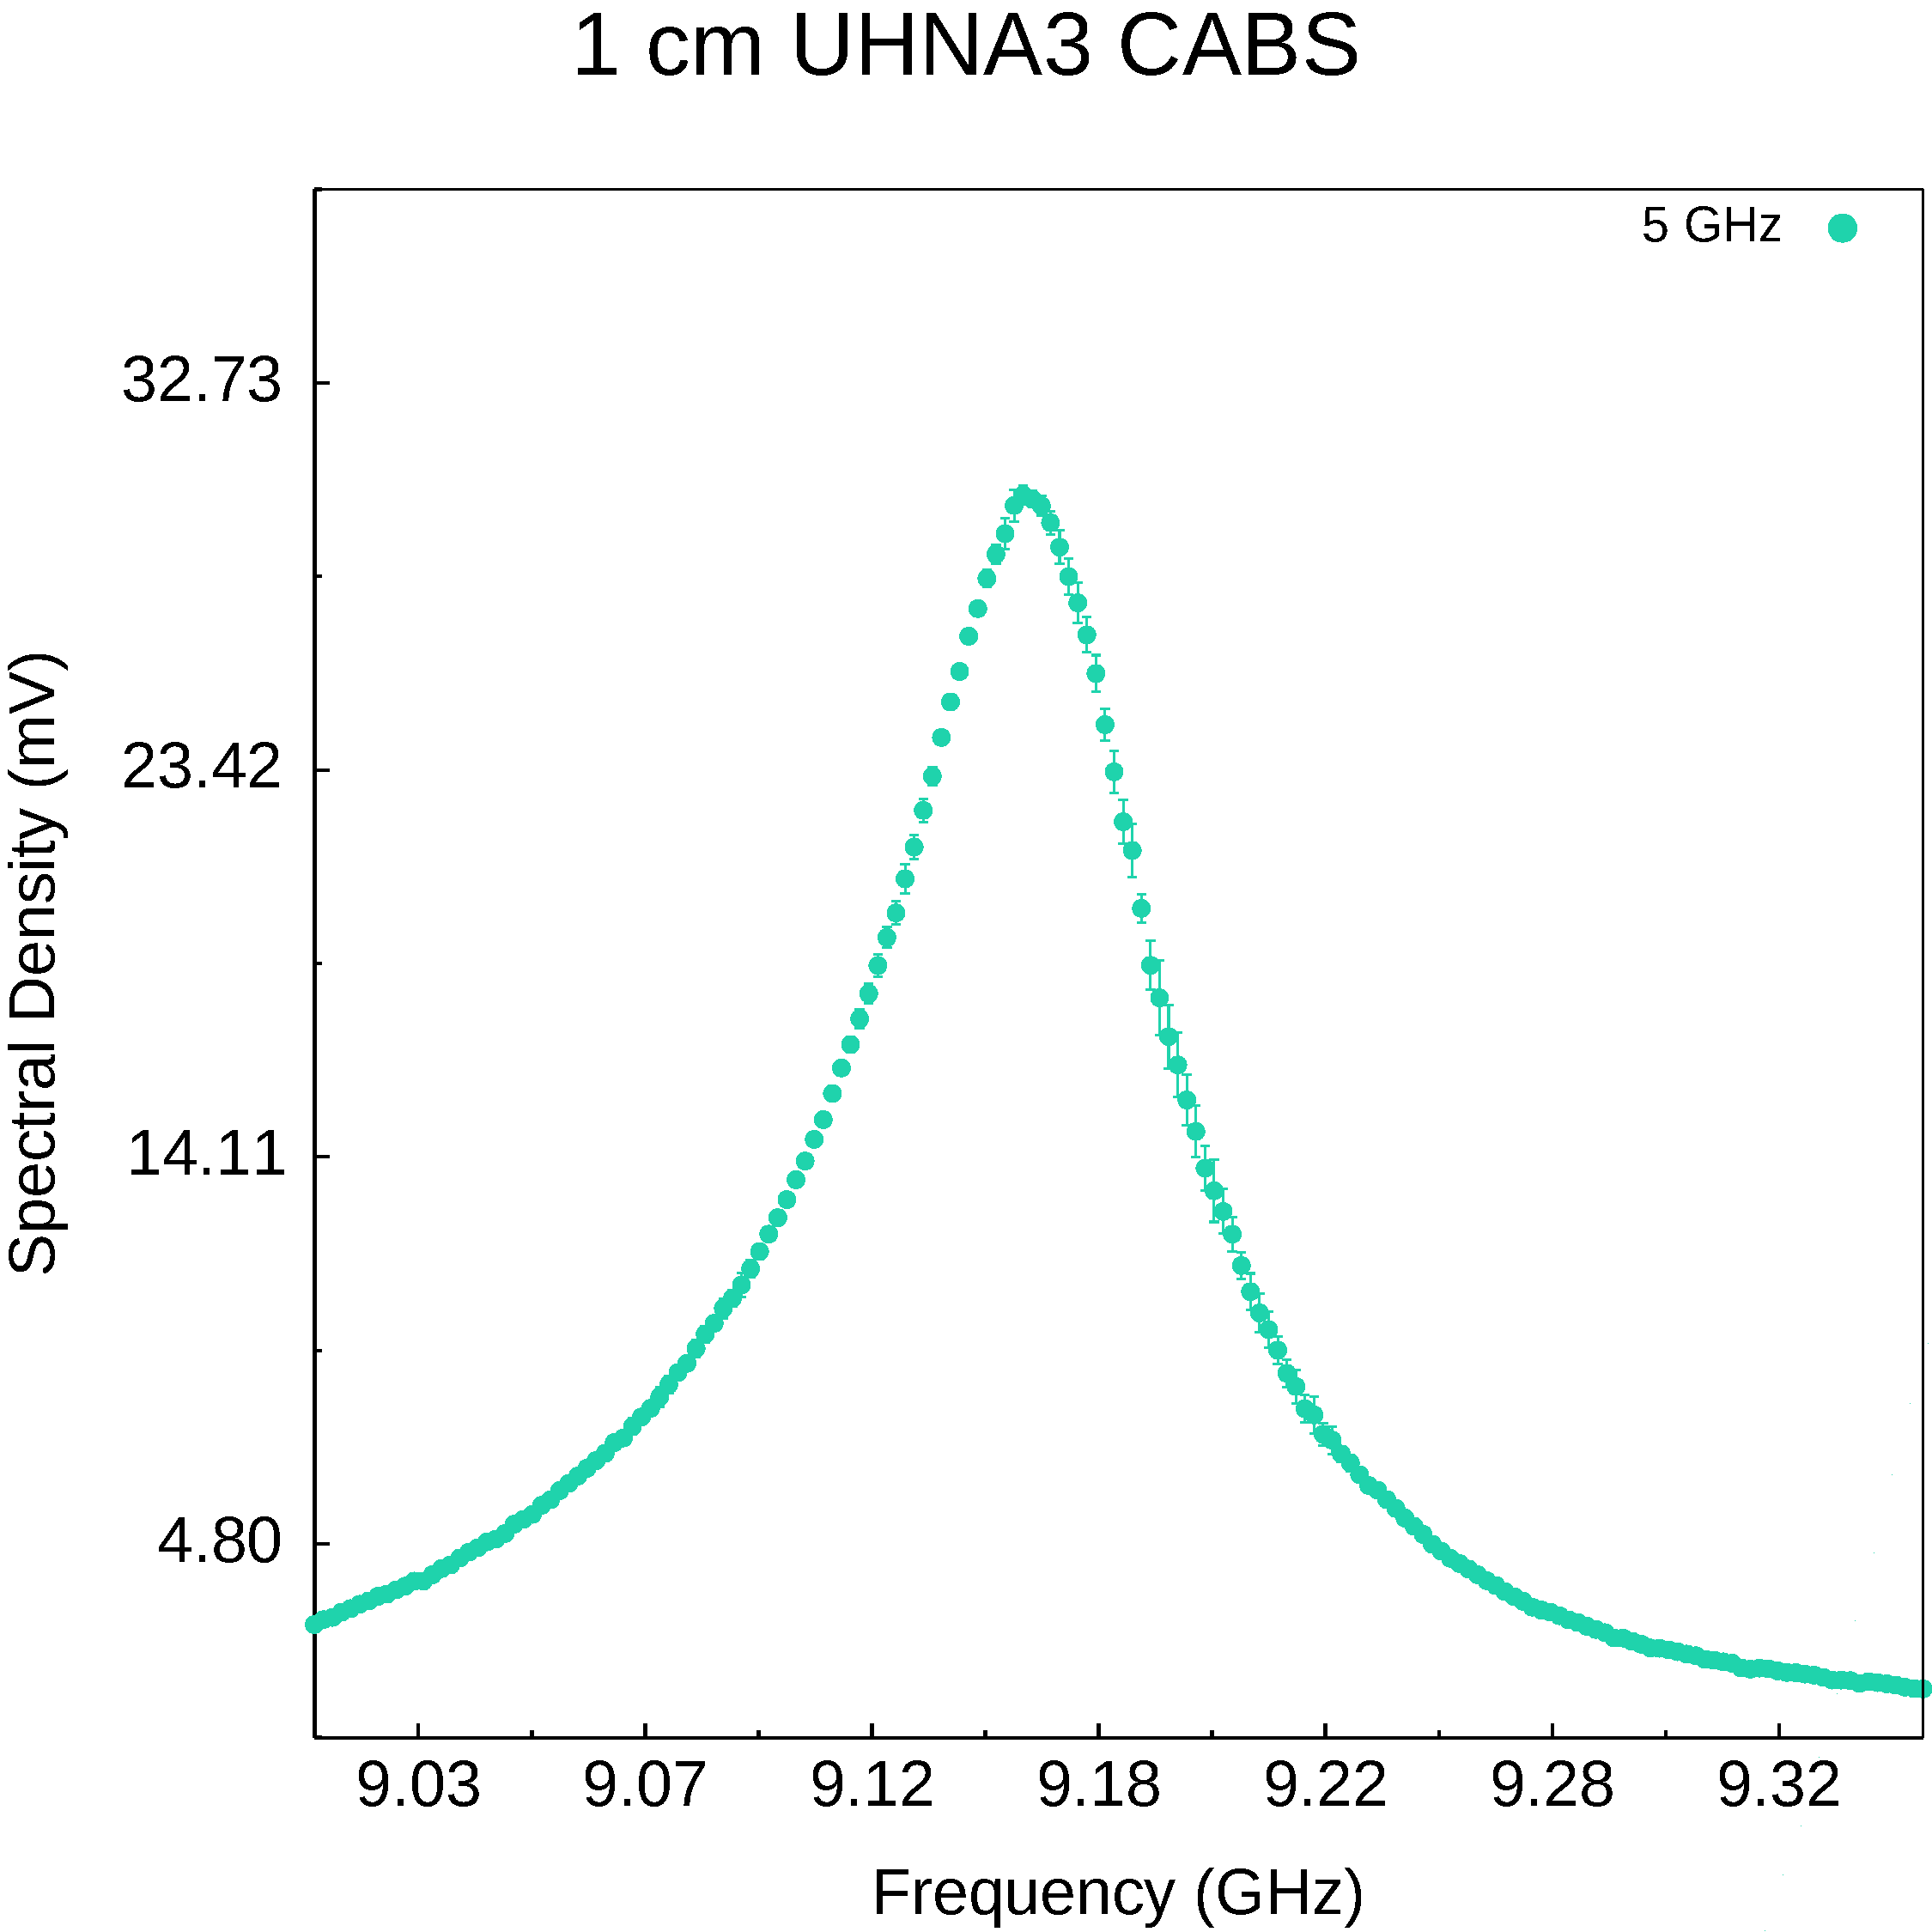
\includegraphics[width=.45\textwidth]{1cmUHNA3.pdf}
  \caption{\SI{1}{\centi\meter} UHNA3}
  \label{fig:1cmUHNA3}
\end{figure}

Fig.~\ref{fig:1cmUHNA3} shows the spectral profile captured for \SI{1}{\centi\meter} of UHNA3 fiber, revealing the expected lorentzian profile consistent with Eq.~\ref{Eq:Effective Brillouin Gain}. The peak amplitude of the spectra occurs at \SI{9.1704}{\giga\hertz}, indicating the Brillouin resonance frequency of the longitudinal traveling-wave mode in the fiber. The FWHM of the measurement is \SI{80}{\mega\hertz} and provides a measure of the phonon dissipation rate. Both values match what is seen in the literature for SBS measurements of UHNA3 fiber.\cite{behunin2015long} The data shown are a background-subtracted average of five successive measurements taken over ten minutes with error bars corresponding to \(1\sigma\) of the mean.

To achieve this measurement of UHNA3 fiber, the instrument design was altered to include only fiber-coupled segments connecting the fiber ports between the two PBSs. We set the pump laser wavelength to \SI{1549.000}{\nano\meter} and the probe laser wavelength to \SI{1549.020}{\nano\meter}, giving a frequency mismatch of approximately \SI{2.5}{\giga\hertz}. The pump--probe mismatch is chosen to be only as large as needed to allow the edge of the pass-band of the probe filter to split the backscattered pump and probe light, thus rejecting any backscattered light from the pump laser and accepting only the backscattered signal from the probe laser. We placed the Stokes filter at \SI{1549.073}{\nano\meter}, an offet of approximately \SI{9.18}{\giga\hertz} from the pump laser to capture the Stokes sideband from the intensity modulator. This corresponds to the center of the measured frequency range and was chosen to allow the Stokes sideband output from the intensity modulator to remain within the pass band of the Stokes filter as the RF signal fed to the intensity modulator is swept through the full measurement range. The probe filter was set to \SI{1549.109}{\nano\meter}, an offset of approximately \SI{11.18}{\giga\hertz} from the probe laser, to capture the Stokes-shifted backscattered signal from the probe. The center frequency of the backscattered signal is of course shifted \SI{9.18}{\giga\hertz} from the probe laser, however an extra offset of \SI{2}{\giga\hertz} is chosen for improved rejection of any pump light as the pass band of our filter extends approximately \SI{2.5}{\giga\hertz} on either side of center.

\begin{figure}[t]
  \centering
  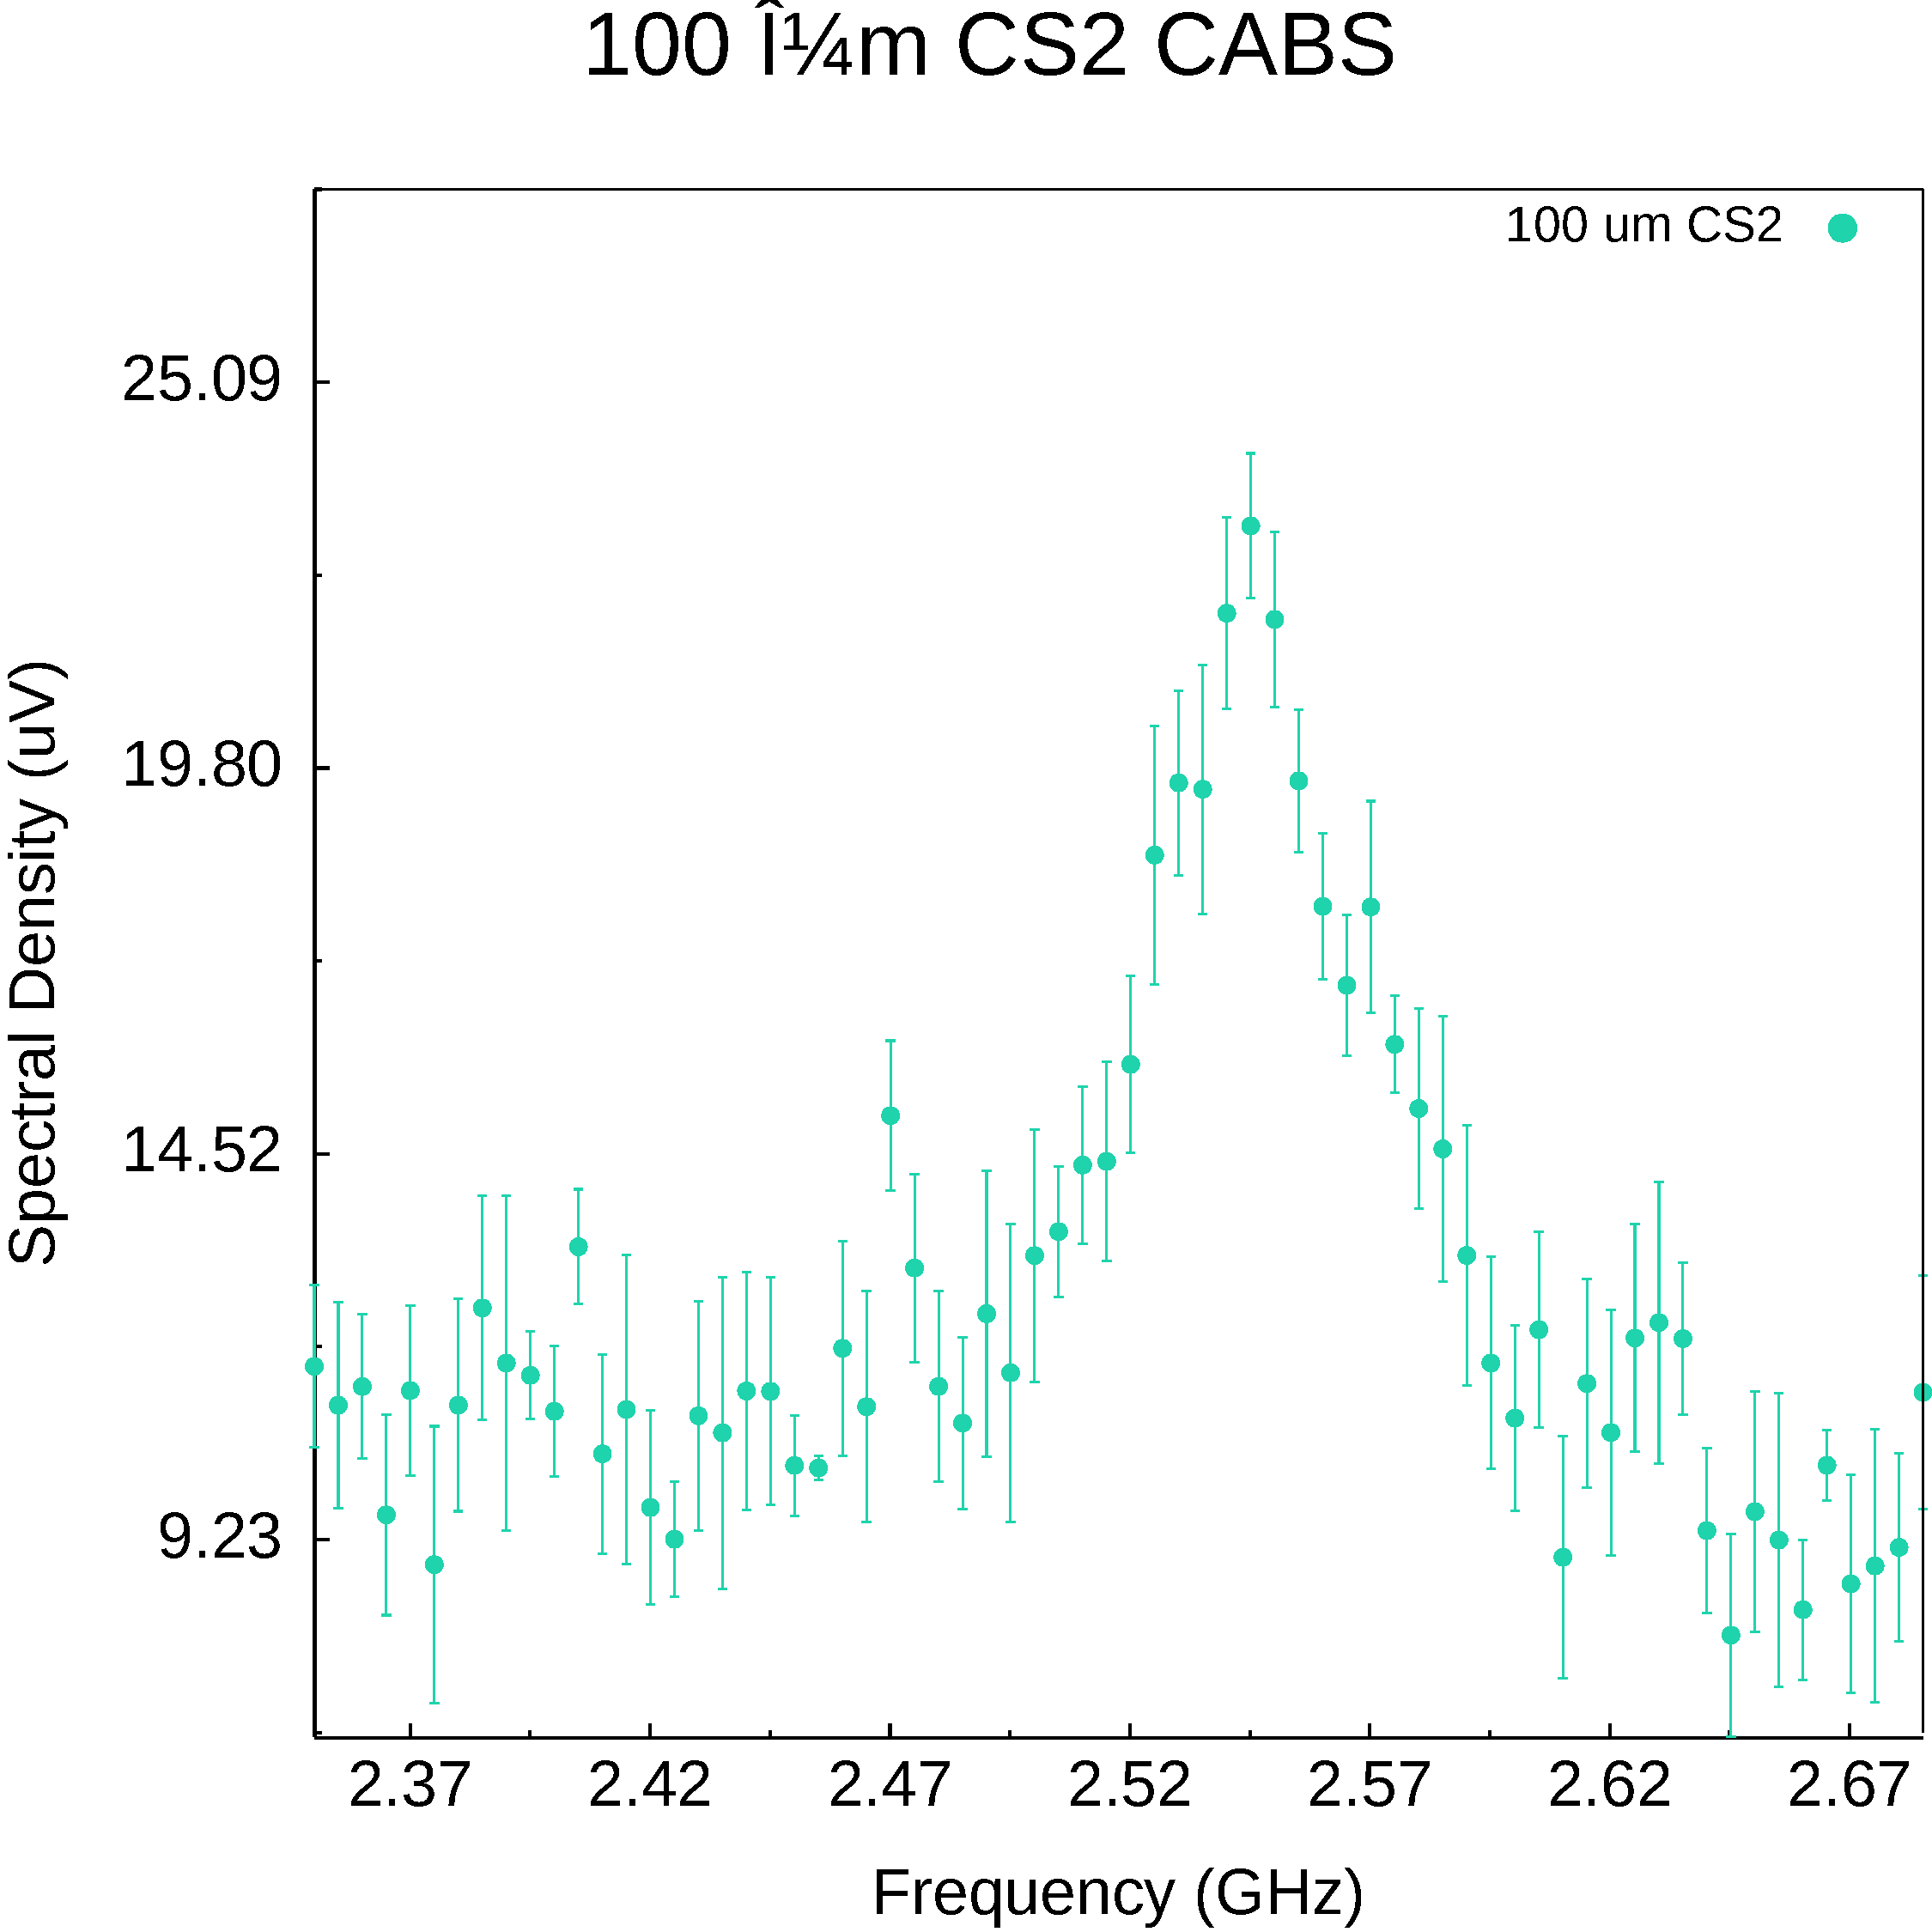
\includegraphics[width=.45\textwidth]{100umCS2.pdf}
  \caption{\SI{100}{\micro\meter} \ce{CS2}}
  \label{fig:100umCS2}
\end{figure}

For a free-space bulk example we target liquid \ce{CS2} for its exceptionally high Brillouin gain factor of \SI{1.5}{\meter\per\giga\watt}.\cite{boyd2020nonlinear} Figure~\ref{fig:100umCS2} reveals the Brillouin signal of bulk \ce{CS2} liquid contained in a \SI{100}{\micro\meter} path length cell. To our knowledge, measurement of longitudinal Brillouin scattering at this scale has not been reported in the literature. A scattered power comparison would reveal that achieving such a measurement using traditional SBS techniques would require excessively high optical powers or cooling the material to cryogenic temperatures, which, of course, would be prohibitive for carbon disulfide in the liquid state.

For this measurement of \ce{CS2}, the pump and probe laser wavelengths were set to \SI{1548.808}{\nano\meter} and \SI{1548.898}{\nano\meter}, respectively. The short path length of the sample significantly broadens \(\Phi\), the \(\mathrm{sinc^2}\) term defining the phasematching bandwidth, allowing for further separation of the pump and probe wavelengths for improved signal isolation without significant reduction in scattered power of the signal produced in the \ce{CS2}. Specifically, the additional pump--probe wavelength separation of \SI{70}{\pico\meter} employed for this measurement compared to the UHNA3 measurement results in a negligible 0.045\% reduction in scattered power. This additional separation contributes meaningfully, however, to improved rejection of pump light by the probe filter and thus higher SNR of the signal.

Placement of the Stokes filter is critical for measurements of materials that give small Brillouin shifts, such as with \ce{CS2} \SI{2.55}{\giga\hertz} shift. We offset our \SI{5}{\giga\hertz} bandwidth Stokes filter an additional \SI{2}{\giga\hertz} to ensure the nearby carrier signal and anti-Stokes sideband from the intensity modulator are rejected and only the Stokes sideband is allowed to pass. For the measurement shown in Fig.~\ref{fig:100umCS2}, this corresponds to a Stokes and probe filter placement of \SI{1548.844}{\nano\meter} and \SI{1548.934}{\nano\meter}, respectively.

% Fig. shows the spectral measurements achieved by the instrument, overlaid with finite-difference simulation data. In Fig. we see the expected lorentzian spectral shape in good alignment with simulation data for guided longitudinal modes in the core of the UHNA3 fiber. In Fig. , however, we see a distortion of this lorentzian shape. This is expected for partially unguided longitudinal modes, such as is the case for a bulk liquid filling the volume of a ...
%
% Fig. \ref{fig:1cmUHNA3} shows a measurement of 1cm of UHNA3 fiber.
%
% First, we measured Brillouin scattering in a 1-centimeter-long UHNA3 fiber at room temperature and with sub-Watt optical power (Fig. ). Figure , clearly displays the Brillouin scattering features with remarkable SNR, highlighting the effectiveness of our apparatus in isolating the backscattered probe light. This observation serves as one of the main showcases of the instrument's capability.
%
% Next, we performed Brillouin scattering measurements on a 4-millimeter-thick bulk carbon disulfide sample in a free-space optics arrangement. The observed spectrum, presented in Figure 2, exhibits well-resolved Brillouin scattering peaks. This successful measurement in a bulk sample demonstrates the versatility and adaptability of our instrument to various experimental configurations, further emphasizing the instrument's capability.
%
% Lastly, we conducted a measurement in a 1-millimeter-long UHNA3 fiber under low-power conditions, with only 10 microwatts of power at the sample. Despite the reduced sample length and low power, the instrument's sensitivity allowed us to observe distinct Brillouin scattering features in the spectrum, as illustrated in Figure 3. This result underscores the potential of our spectrometer for nanoscale measurements and serves as a demonstration of the instrument's sensitivity, defining the sensitivity floor of the apparatus.
%
% These three observations collectively showcase the high sensitivity, broad applicability, and impressive capabilities of our coherent stimulated phonon spectrometer in measuring Brillouin scattering across different sample types, scales, and power levels.

\subsection*{Phase Matching Bandwidth}
\label{Results:Phase Matching Characterization}

To characterize the phase matching tolerance of the instrument for a given length of sample, we performed an additional experiment whereby we took a series of measurements of \SI{1}{\centi\meter} of UHNA3 at constant optical powers while letting the detuning of the pump and probe lasers vary. In the language of Eq.~\ref{Eq:Theoretical Framework:Scattered Power}, this experiment holds \(G_B\), \(L\), \(P_P\), \(P_S\), and \(P_{Pr}\) constant while letting \(\Delta k\) vary. For the experiment to support the validation of Eq.~\ref{Eq:Theoretical Framework:Scattered Power}, we would expect the peak amplitudes of these measurements to trace out a \(\mathrm{sinc^2}\) profile, also given by Eq.~\ref{Eq:Phi}. Fig.~\ref{fig:Phase-Match} shows the results of this experiment, in which 75 measurements performed between \SI{5}{\giga\hertz} and \SI{42}{\giga\hertz} pump--probe frequency separation at \SI{0.5}{\giga\hertz} intervals. We found peak amplitudes by fitting each spectra with a Fano profile (see the proceeding \textit{Fano-Resonant Asymmetries at Small Signals} subsection) and are represented by a point in Fig.~\ref{fig:Phase-Match}. The theoretical \(\mathrm{sinc^2}\) function for the parameters used in the experiment (listed in Table~\ref{tab:Phase-Match Parameters} in Appendix~\ref{}) is shown on the plot with a solid red line.

%Describe adjustments and/or explain deviations from pure sinc^2 (noise floor, Fano effects, L uncertainty, etc.), or reference Fano section

\begin{figure}[t]
\centering
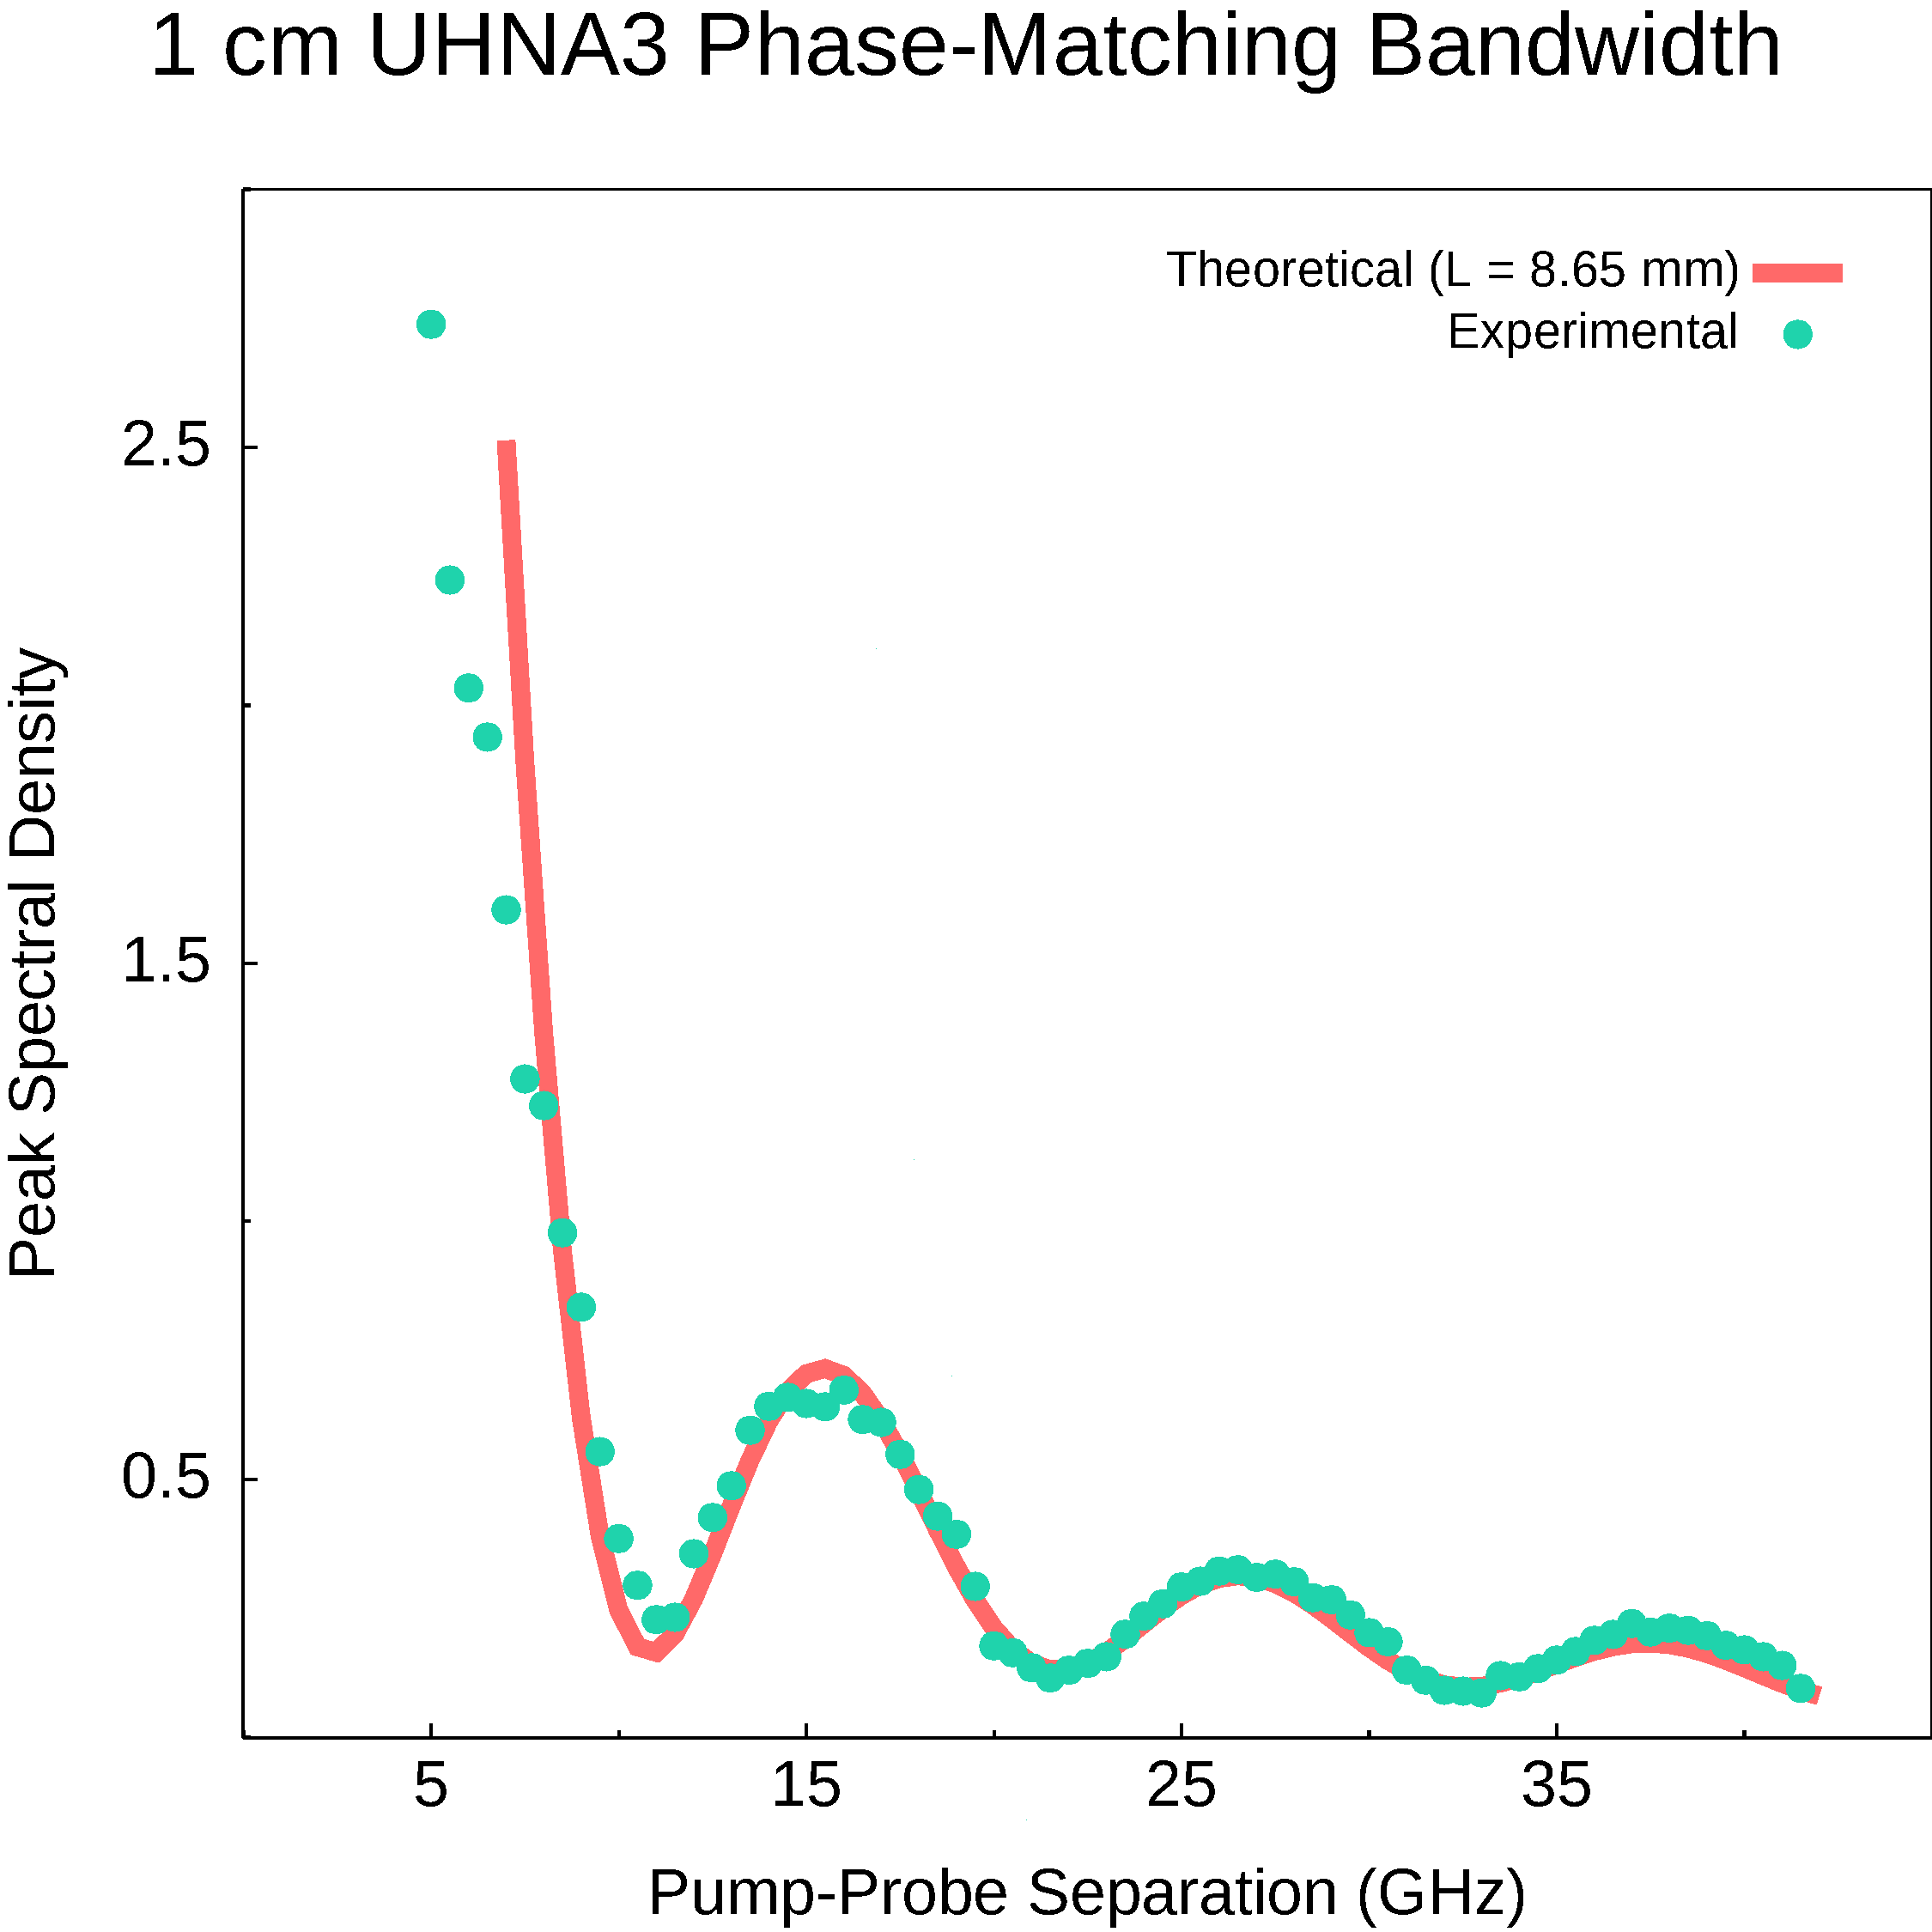
\includegraphics[width=.45\textwidth]{Phase-Match.pdf}
\caption{Phase-matching \(\mathrm{sinc^2}\) func}
\label{fig:Phase-Match}
\end{figure}

\subsection*{Fano-Resonant Asymmetries at Small Signals}
\label{Results:Fano-Resonant Asymmetries at Small Signals}

Under certain conditions where the resonant Brillouin amplitude approaches the background continuum level, we observe an asymmetric, Fano‐type lineshape\cite{fano1961effects, limonov2017fano, limonov2021fano, kroner2008nonlinear}. These Fano distortions can shift the apparent peak frequency, complicate simple Lorentzian fitting, and affect the extracted linewidth in small‐signal measurements.\cite{...} To properly handle these occurances, it is necessary to understand when they are likely to arise with this technique and how they may be corrected for or controlled. Fano resonances arise when a discrete resonance (in our case, the Brillouin mode) interferes with a continuum background (e.g., noise floor or broad, non‐resonant scattering). When the resonance amplitude is no longer much larger than the continuum, the interference leads to an asymmetric lineshape described by the Fano formula\cite{fano1961effects},

\begin{equation}
I(\omega) \propto \frac{(q + \epsilon)^2}{1 + \epsilon^2},
\end{equation}

where \(\epsilon \equiv (\Omega - \Omega_{B})/(\Gamma_{B}/2)\) is the dimensionless detuning from the Brillouin peak (measured in half the spectral linewidth) and \(q\) is the Fano asymmetry parameter.

We first noticed this behavior appearing in our small-length \ce{CS2} data, where a small shift in probe wavelength revealed an asymmetric lineshape. For the measurements of \SI{100}{\micro\meter} \ce{CS2} (Fig.~\ref{fig:100umCS2}) and \SI{1}{\centi\meter} UHNA3 fiber at low power (Fig.~\ref{fig:5fWSensitivity}), the amplitude of the resonant Brillouin peak is on the order of that of the non‐resonant continuum, giving a strong chance for Fano interference. Whenever \(\tfrac{I_{\text{res}}}{I_{\text{bkg}}}\approx 1\), the parameter \(q\) can become finite (rather than \(\pm \infty\) in the limit that the background is negligible), and Fano interference arises. To explore this further, we performed a similar phase-matching experiment as was done for \SI{1}{\centi\meter} UHNA3 (see Phase Matching Bandwidth subsection), this time with \SI{1}{\milli\meter} of \ce{CS2}. Results from this are presented in Appendix~\ref{Appendix:Fano} and offer a striking example of line shapes with pronounced asymmetry and featuring clear characteristic morphologies associated with various values and signs of \(q\). These pronounced distortions in spectral line shape for small signal measurements underscore the role of Fano interference in small resonant amplitudes relative to the background.

As our instrument is well suited to measuring samples of length \(<\SI{10}{\meter}\) and low Brillouin gain, typical signal amplitudes are often small and may sometimes approach the order of the background continuum amplitude. For this reason, Fano effects may more often be present with this technique and must be handled appropriately, such as fitting data with a Fano profile as opposed to a Lorentzian to ensure accurate capture of relevant parameters such as linewidth and peak amplitude. Beyond fitting and parameter extraction, it is important to be mindful that these effects are likely to occur in ambitious measurements at the limits of equipment sensitivity. Expectation and proper handling of Fano effects in measurements of this nature ensures that they may be more easily recognized and confirmed, as the data is likely to present a spectrum that deviates considerably from the standard Lorentzian. In some cases, and of particular interest for ambitious measurements, Fano interference may even \textit{boost} the measured peak above its nominal amplitude—i.e., ‘amplify’ it—when \(q < 0\). This peak-boosting effect occurs when the scattered Brillouin signal \textit{lags} the background continuum in phase, resulting in a negative \(q\).

In principle, the Fano lineshape can exhibit a higher peak amplitude than a pure Lorentzian if the discrete Brillouin response interferes constructively with the background near resonance. However, this does not represent net energy gain, since it is an interference effect rather than a true amplification mechanism. Depending on the phase relationship and the background noise level, the observed peak may be taller (enhancing local amplitude), but the net SNR may or may not improve globally, since the background continuum also contributes noise. In any case, our technique permits tuning of the probe wavelength to tailor the phase of the Brillouin signal relative to the background continuum for optimal Fano interference for a given system and measurement. Remarkably, this can be done without giving up independent control of the phase matching bandwidth. This can be achieved through simultaneous adjustment of the pump laser wavelength in step with the probe such that the probe wavelength is Fano-optimized and the desired pump--probe detuning is preserved.

In the phase-matching bandwidth experiment performed on \SI{1}{\centi\meter} UHNA3 (Fig.~\ref{fig:Phase-Match} and described in Phase Matching Bandwidth subsection), several factors contribute to a slight deviation from the simple theory of a pure \(\mathrm{sinc^2}\) function, including noise floor, alignment drifts, fiber dispersion, among possible others. We largely see the \(\mathrm{sinc^2}\) dependence, however near the troughs of the \(\mathrm{sinc^2}\) function and for greater pump-probe detunings, the measured peaks become quite weak, and a slight spectral asymmetry emerges (see Appendix~\ref{Appendix:Fano}). This is consistent with a Fano‐type distortion, wherein the signal amplitude is comparable to the underlying continuum, leading to an interference phenomenon that slightly skews the measured peak. Because of the Fano line shape, the peak amplitude from the spectral trace is not exactly at the Lorentzian center and a naive Lorentzian fit would thus not accurately capture the peak amplitude of these greater pump--probe detunings. We corrected for this by fitting a standard Fano profile, which accurately captures the peak amplitudes. Comparing a pure Lorentzian vs.\ a Fano fit in the limiting data sets indicates that ignoring the Fano effect overestimates the peak amplitude by ~5–10\%. However, even with a good fit, as described earlier, the Fano-resonant effects serve to amplify or diminish the underlying Brillouin response as a function of the sign of the Fano asymmetry parameter \(q\) for each set (e.g. whether the Brillouin response slightly lags (\(q < 0\)) or leads (\(q > 0\)) the broad background continuum in phase, respectively, as determined by the wavelength of the Probe laser).

% ...~5–10\% and shifts the center frequency by up to __.

\section{Conclusion}
\label{Conclusion}

In conclusion, we have introduced a coherently stimulated Brillouin spectrometer utilizing a detuned pump-probe design to achieve high sensitivity and room-temperature operation in \si{\micro\meter}-scale samples. This approach successfully overcomes the spatial resolution limitations imposed by conventional SBS methods, demonstrating sub-\SI{10}{\femto\watt} sensitivity in UHNA3 fiber and enabling Brillouin measurements in bulk liquid carbon disulfide with unprecedented efficiency. By relaxing phase-matching constraints, this instrument opens new possibilities for characterizing nanoscale material properties and developing nano-acousto-optic devices in standard laboratory settings without the need for cryogenic environments. Moving forward, our methodology could facilitate advancements in high-resolution phonon spectroscopy and inspire further innovations in the study of material mechanics at the microscale, reinforcing the broader applicability of Brillouin-based techniques across materials science, photonics, and sensing technologies.


\begin{acknowledgments}
The authors acknowledge the developers of the Go programming language (\href{https://go.dev}{https://go.dev}) for providing the tools used in data processing and visualization.
\end{acknowledgments}

% Switch to appendices in one column
\clearpage % Ends the current page and all its floating elements.
\onecolumngrid % Switches to one-column format.

\begin{titlepage}
\centering
\vspace*{\stretch{1}}
{\Large Appendix:\\[10pt] A Coherently Stimulated Brillouin Spectrometer\par}
\vspace{\stretch{3}}
\end{titlepage}

\clearpage
\onecolumngrid
\clearpage

\appendix

\section{Coupled-Wave Equations}
\label{Appendix:Coupled-Wave Equations}

Here we derive the coupled wave equations that describe coherent stimulated Brillouin scattering involving a pump, Stokes, probe, and backscattered optical field given respectively by
\\
\begin{equation}
    \tilde{E}_{P}(z,t) = A_{P}e^{i(k_{P}z - \omega_{P}t)} + c.c.,
    \label{eq:Pump optical field}
\end{equation}
\\
\begin{equation}
    \tilde{E}_{S}(z,t) = A_{S}e^{i(k_{S}z - \omega_{S}t)} + c.c.,
    \label{eq:Stokes optical field}
\end{equation}
\\
\begin{equation}
    \tilde{E}_{Pr}(z,t) = A_{Pr}e^{i(k_{Pr}z - \omega_{Pr}t)} + c.c.,
    \label{eq:Probe optical field}
\end{equation}
\\
\begin{equation}
    \tilde{E}_{Sig}(z,t) = A_{Sig}e^{i(k_{Sig}z - \omega_{Sig}t)} + c.c.,
    \label{eq:Signal optical field}
\end{equation}
\\
\noindent and a common acoustic field given by
\\
\begin{equation}
    \tilde{\rho}(z,t) = \rho_{0} + \rho(z,t)e^{i(qz - \Omega t)} + c.c.,
    \label{eq:acoustic field}
\end{equation}
\\
\noindent where \(\Omega = \omega_{P} - \omega_{S}\) and \(q = k_{P} - k_{S} = 2k_{P}\).


\subsection{Acoustic Field}
\label{Coupled-Wave Equations:Acoustic Field}

As in the case of SBS\cite{boyd2020nonlinear}, we start by assuming that the material obeys the acoustic wave equation,
\\
\begin{equation}
    \frac{\partial^{2}\tilde{\rho}}{\partial t^{2}} - \Gamma^{\prime}\nabla^{2}\frac{\partial\tilde{\rho}}{\partial t} - v_{s}^{2}\nabla^{2}\tilde{\rho} = \nabla\cdot\vec{f},
    \label{eq:acoustic wave equation}
\end{equation}
\\
\noindent where \(v_{s}\) is the sound speed in the material and \(\Gamma^{\prime}\) is a damping parameter given by
\\
\begin{equation}
    \Gamma^{\prime} = \frac{1}{\rho}\left[\frac{4}{3}\eta_{s} + \eta_{b} + \frac{\kappa}{C_{p}}(\gamma - 1)\right],
\end{equation}
\\
\noindent where \(\eta_{s}\) and \(\eta_{b}\) are the shear and bulk viscosity coefficients of the material, respectively. The source term on the right side of Eq.~\ref{eq:acoustic wave equation} is the divergence of the electrostrictive force:
\\
\begin{equation}
    \vec{f} = \nabla p_{st} = \nabla \cdot \Bigg[-\frac{1}{2}\epsilon_{0}\gamma_{e}\Big(\langle\tilde{E}_{P} \cdot \tilde{E}_{S}\rangle + \langle\tilde{E}_{Pr} \cdot \tilde{E}_{Sig}\rangle\Big)\Bigg],
\end{equation}
\\
which yields, after applying the slowly varying amplitude approximation,
\\
\begin{equation}
    \nabla\cdot\vec{f} = \epsilon_{0}\gamma_{e}q^{2}(A_{P}A_{S}^{*} + A_{Pr}A_{Sig}^{*})e^{i\Delta kz},
\end{equation}
\\
Where \(\Delta k = (k_{Pr} - k_{Sig}) - (k_{P} - k_{S})\) is the phase mismatch between the four optical fields. Only two electrostrictive terms survive after accounting for the orthogonal polarization of the pump and Stokes fields with respect to that of the probe and backscattered signal. Inserting this electrostrictive force term and the acoustic field (Eq.~\ref{eq:acoustic field}) into Eq.~\ref{eq:acoustic wave equation}, and assuming a slowly varying acoustic amplitude, we find
\\
\begin{equation}
    -2i\Omega\frac{\partial\rho}{\partial t} - \Gamma^{\prime}2iq^{2}\Omega\rho - 2iqv_{s}^{2}\frac{\partial\rho}{\partial z} = \epsilon_{0}\gamma_{e}q^{2}(A_{P}A_{S}^{*} + A_{Pr}A_{Sig}^{*})e^{i\Delta kz},
\end{equation}
\\
which can be restated in terms of the Brillouin linewidth, \(\Gamma_{B} = q^{2}\Gamma^{\prime}\), as
\\
\begin{equation}
    -2i\Omega\frac{\partial\rho}{\partial t} - 2i\Omega\Gamma_{B}\rho - 2iqv_{s}^{2}\frac{\partial\rho}{\partial z} = \epsilon_{0}\gamma_{e}q^{2}(A_{P}A_{S}^{*} + A_{Pr}A_{Sig}^{*})e^{i\Delta kz}.
    \label{eq:in terms of Brillouin linewidth}
\end{equation}
\\
Given the phonon dispersion relations \(\Omega_{B} = |q_{B}|v_{s}\) and \(\Omega^{2} = q^{2}\left(v^{2} - i\Omega\Gamma^{\prime}\right)\), Eq.~\ref{eq:in terms of Brillouin linewidth} can be rewritten as
\\
\begin{equation}
    -2i\Omega\frac{\partial\rho}{\partial t} + \left(\Omega^{2} - \Omega^{2} - i\Omega\Gamma_{B}\right)\rho - 2iqv_{s}^{2}\frac{\partial\rho}{\partial z} = \epsilon_{0}\gamma_{e}q^{2}(A_{P}A_{S}^{*} + A_{Pr}A_{Sig}^{*})e^{i\Delta kz}.
    \label{eq:in terms of Omega_B}
\end{equation}
\\
We take the common assumption that the phonon propagation distance is small compared to the distance over which the source term varies significantly, which allows the spatial derivative term in Eq.~\ref{eq:in terms of Omega_B} to be dropped. We further assume steady-state conditions such that the time derivative term also vanishes, leaving
\\
\begin{equation}
    (\Omega^{2}_{B} - \Omega^{2} - i\Omega\Gamma_{B})_{\rho} = \epsilon_{0}\gamma_{e}q^{2}(A_{P}A_{S}^{*} + A_{Pr}A_{Sig}^{*})e^{i\Delta kz}.
\end{equation}
\\
We thus find the acoustic field amplitude to be
\\
\begin{equation}
    \rho(z,t) = \epsilon_{0}\gamma_{e}q^{2}\frac{(A_{P}A_{S}^{*} + A_{Pr}A_{Sig}^{*})e^{i\Delta kz}}{\Omega_{B}^{2} - \Omega^{2} - i\Omega\Gamma_{B}}.
    \label{eq:Acoustic field amplitude}
\end{equation}


\subsection{Optical Fields}
\label{Coupled-Wave Equations:Optical Fields}

We now turn to the spatial evolution of the optical fields, described by the wave equation,
\\
\begin{equation}
    \frac{\partial^{2}\tilde{E}_{i}}{\partial z^{2}} - \frac{n^{2}}{c^{2}}\frac{\partial^{2}\tilde{E}_{i}}{\partial t^{2}} = \frac{1}{\epsilon_{0}c^{2}}\frac{\partial^{2}\tilde{P}_{i}}{\partial t^{2}},
    \label{eq:Wave equation}
\end{equation}
\\
where \(i\) denotes the four optical fields, namely: pump, Stokes, probe, and the backscattered signal. The total nonlinear polarization that gives rise to the source term in the wave equation is given by
\\
\begin{equation}
    \tilde{P} = \epsilon_{0}\Delta\chi\tilde{E} = \epsilon_{0}\Delta\epsilon\tilde{E} = \epsilon_{0}\rho^{-1}\gamma_{e}\tilde{\rho}\tilde{E}.
\end{equation}
\\
The parts of \(\tilde{P}\) that can act as phase-matched source terms for the optical fields are
\\
\begin{equation}
    \tilde{P}_{P} = p_{P}e^{i(k_{P}z - \omega_{P} t)} + c.c. = \frac{1}{2}\epsilon_{0}\rho_{0}^{-1}\gamma_{e}\rho A_{S}e^{i(k_{P}z - \omega_{P} t)},
    \label{eq:Pump phase-matched source term}
\end{equation}
\\
\begin{equation}
    \tilde{P}_{S} = p_{S}e^{i(-k_{S}z - \omega_{S} t)} + c.c. = \frac{1}{2}\epsilon_{0}\rho_{0}^{-1}\gamma_{e}\rho^{*} A_{P}e^{i(-k_{S}z - \omega_{S} t)},
    \label{eq:Stokes phase-matched source term}
\end{equation}
\\
\begin{equation}
    \tilde{P}_{Pr} = p_{Pr}e^{i(k_{Pr}z - \omega_{Pr} t)} + c.c. = \frac{1}{2}\epsilon_{0}\rho_{0}^{-1}\gamma_{e}\rho A_{Sig}e^{i(k_{Pr}z - \omega_{Pr} t)}e^{i\Delta kz},
    \label{eq:Probe phase-matched source term}
\end{equation}
\\
\begin{equation}
    \tilde{P}_{Sig} = p_{Sig}e^{i(-k_{Sig}z - \omega_{Sig} t)} + c.c. = \frac{1}{2}\epsilon_{0}\rho_{0}^{-1}\gamma_{e}\rho^{*} A_{Pr}e^{i(-k_{Sig}z - \omega_{Sig} t)}e^{-i\Delta kz}.
    \label{eq:Signal phase-matched source term}
\end{equation}
\\
Inserting the optical fields (Eqs.~\ref{eq:Pump optical field}-\ref{eq:Signal optical field}) and phase-matched source terms (Eqs.~\ref{eq:Pump phase-matched source term}-\ref{eq:Signal phase-matched source term}) into Eq.~\ref{eq:Wave equation}, we obtain
\\
\begin{equation}
    \frac{\partial A_{P}}{\partial z} + \frac{n}{c}\frac{\partial A_{P}}{\partial t} = \frac{i\omega_{P}\gamma_{e}}{2nc\rho_{0}}\rho A_{2},
\end{equation}
\\
\begin{equation}
    -\frac{\partial A_{S}}{\partial z} + \frac{n}{c}\frac{\partial A_{S}}{\partial t} = \frac{i\omega_{S}\gamma_{e}}{2nc\rho_{0}}\rho^{*}A_{P},
\end{equation}
\\
\begin{equation}
    \frac{\partial A_{Pr}}{\partial z} + \frac{n}{c}\frac{\partial A_{Pr}}{\partial t} = \frac{i\omega_{Pr}\gamma_{e}}{2nc\rho_{0}}\rho A_{Sig},
\end{equation}
\\
\begin{equation}
    -\frac{\partial A_{Sig}}{\partial z} + \frac{n}{c}\frac{\partial A_{Sig}}{\partial t} = \frac{i\omega_{Sig}\gamma_{e}}{2nc\rho_{0}}\rho^{*}A_{Pr},
\end{equation}
\\
We again assume steady-state conditions, allowing the time derivative term to be dropped. Plugging in the acoustic field amplitude (Eq.~\ref{eq:Acoustic field amplitude}), we arrive at the coupled-amplitude wave equations for the optical fields,
\\
\begin{equation}
    \frac{\partial A_{P}}{\partial z} = \frac{i\epsilon_{0}\omega_{P} q^{2}\gamma_{e}^{2}}{2nc\rho_{0}}\frac{(A_{P}|A_{S}|^{2} + A_{Pr}A_{Sig}^{*}A_{S})e^{i\Delta kz}}{\Omega_{B}^{2} - \Omega^{2} - i\Omega\Gamma_{B}},
    \label{eq:Pump coupled-amplitude wave equation}
\end{equation}
\\
\begin{equation}
    \frac{\partial A_{S}}{\partial z} = -\frac{i\epsilon_{0}\omega_{S} q^{2}\gamma_{e}^{2}}{2nc\rho_{0}}\frac{(|A_{P}|^{2}A_{S}^{*} + A_{Pr}A_{Sig}^{*}A_{P})e^{-i\Delta kz}}{\Omega_{B}^{2} - \Omega^{2} + i\Omega\Gamma_{B}},
\end{equation}
\\
\begin{equation}
    \frac{\partial A_{Pr}}{\partial z} = \frac{i\epsilon_{0}\omega_{Pr} q^{2}\gamma_{e}^{2}}{2nc\rho_{0}}\frac{(A_{P}A_{S}^{*}A_{Sig} + A_{Pr}|A_{Sig}|^{2})e^{i\Delta kz}}{\Omega_{B}^{2} - \Omega^{2} - i\Omega\Gamma_{B}},
\end{equation}
\\
\begin{equation}
    \frac{\partial A_{Sig}}{\partial z} = -\frac{i\epsilon_{0}\omega_{Sig} q^{2}\gamma_{e}^{2}}{2nc\rho_{0}}\frac{(A_{P}A_{S}^{*}A_{Pr} + |A_{Pr}|^{2}A_{Sig}^{*})e^{-i\Delta kz}}{\Omega_{B}^{2} - \Omega^{2} + i\Omega\Gamma_{B}}.
    \label{eq:Signal coupled-amplitude wave equation}
\end{equation}
\\
We drop the very small signal amplitude terms on the right side of Eqs.~\ref{eq:Pump coupled-amplitude wave equation}-\ref{eq:Signal coupled-amplitude wave equation} and integrate each along the effective length to get the amplitudes,
\\
\begin{equation}
  A_{P} = \frac{i\epsilon_{0}\omega_{P}q^{2}\gamma_{e}^{2}}{2nc\rho_{0}}\frac{A_{P}|A_{S}|^{2}}{\Omega_{B}^{2} - \Omega^{2} - i\Omega\Gamma_{B}} \frac{e^{i\Delta kL} - 1}{i\Delta k},
\end{equation}
\\
\begin{equation}
  A_{S} = -\frac{i\epsilon_{0}\omega_{S}q^{2}\gamma_{e}^{2}}{2nc\rho_{0}}\frac{|A_{P}|^{2}A_{S}^{*}}{\Omega_{B}^{2} - \Omega^{2} + i\Omega\Gamma_{B}} \frac{e^{-i\Delta kL} - 1}{-i\Delta k},
\end{equation}
\\
\begin{equation}
  A_{Pr} = \frac{i\epsilon_{0}\omega_{Pr}q^{2}\gamma_{e}^{2}}{2nc\rho_{0}}\frac{A_{P}A_{S}^{*}A_{Sig}}{\Omega_{B}^{2} - \Omega^{2} - i\Omega\Gamma_{B}} \frac{e^{i\Delta kL} - 1}{i\Delta k},
\end{equation}
\\
\begin{equation}
  A_{Sig} = -\frac{i\epsilon_{0}\omega_{Sig}q^{2}\gamma_{e}^{2}}{2nc\rho_{0}}\frac{A_{P}A_{S}^{*}A_{Pr}}{\Omega_{B}^{2} - \Omega^{2} + i\Omega\Gamma_{B}} \frac{e^{-i\Delta kL} - 1}{-i\Delta k}.
  \label{eq:Signal amplitude}
\end{equation}
\\
We focus on the signal amplitude given by Eq.~\ref{eq:Signal amplitude}, noting that close to resonance, the denomenator of the middle term containing \(\Omega\) can be approximated as,
\\
\begin{equation}
\Omega_{B}^{2} - \Omega^{2} + i\Omega\Gamma_{B} \approx \Omega_{B}(\Omega - \Omega_{B} + i\Gamma_{B}),
\end{equation}
\\
giving
\\
\begin{equation}
  A_{Sig} = -\frac{i\epsilon_{0}\omega_{Sig}q^{2}\gamma_{e}^{2}}{2nc\rho_{0}}\frac{A_{P}A_{S}^{*}A_{Pr}}{\Omega_{B}(\Omega - \Omega_{B} + i\Gamma_{B})} \frac{e^{-i\Delta kL} - 1}{-i\Delta k},
  \label{eq:resonance}
\end{equation}
\\
and in fact on resonance the expression reduces to
\\
\begin{equation}
  A_{Sig} = -\frac{i\epsilon_{0}\omega_{Sig}q^{2}\gamma_{e}^{2}}{2nc\rho_{0}}\frac{A_{P}A_{S}^{*}A_{Pr}}{\Omega_{B}i\Gamma_{B}} \frac{e^{-i\Delta kL} - 1}{-i\Delta k}.
\end{equation}
\\
Using \(q = 2k_{P} = 2\omega n/c\) and \(q = \Omega_{B}/v_{s}\), we can express the leading terms as
\\
\begin{equation}
  A_{Sig} = -\frac{\epsilon_{0}\omega^{2}\gamma_{e}^{2}}{c^{2}v_{s}\rho_{0}\Gamma_{B}}A_{P}A_{S}^{*}A_{Pr} \frac{e^{-i\Delta kL} - 1}{-i\Delta k},
\end{equation}
\\
where we have dropped the signal designator on \(\omega\). Defining the Brillouin gain factor, \(g_{0}\), as Boyd does,
\\
\begin{equation}
  g_{0} = \frac{\gamma_{e}^{2}\omega^{2}}{nvc^{3}\rho_{0}\Gamma_{B}},
\end{equation}
reduces this expression to
\\
\begin{equation}
  A_{Sig} = -\epsilon_{0}ncg_{0}A_{P}A_{S}^{*}A_{Pr} \frac{e^{-i\Delta kL} - 1}{-i\Delta k}.
\end{equation}
\\
The intensity of the backscattered signal is given by the magnitude of the time-averaged Poynting vector, given by
\\
\begin{equation}
  I_{i} = 2n\epsilon_{0}c|A_{i}|^{2}, \qquad i = 1,2,3,...
\end{equation}
\\
which produces for the signal intensity
\\
\begin{equation}
  I_{Sig} = 2\epsilon_{0}nc(\epsilon_{0}ncg_{0})^{2}|A_{P}|^{2}|A_{S}^{*}|^{2}|A_{Pr}|^{2}\left|\frac{e^{-e\Delta kL} - 1}{-i\Delta k}\right|^{2}
  = 2\epsilon_{0}^{3}\epsilon_{0}n^{3}c^{3}g_{0}^{2}\frac{I_{P}}{2\epsilon_{0}nc}\frac{I_{S}}{2\epsilon_{0}nc}\frac{I_{Pr}}{2\epsilon_{0}nc}\left|\frac{e^{-e\Delta kL} - 1}{-i\Delta k}\right|^{2}.
\end{equation}
\\
The squared modulus term containing \(\Delta k\) can be reduced as
\\
\begin{gather}
  \bigg|\frac{e^{-i\Delta kL} - 1}{-i\Delta k}\bigg|^{2} = \frac{(e^{-i\Delta kL} - 1)(e^{i\Delta kL} - 1)}{(\Delta k)^{2}} = \frac{L^{2}}{(\Delta kL)^{2}}\Bigg[ 2 - 2\Bigg(\frac{e^{i\Delta kL} + e^{-1\Delta kL}}{2}\Bigg)\Bigg] \notag \\ \notag \\
  = \frac{2L^{2}(1 - cos\Delta kL)}{(\Delta kL)^{2}} = \frac{4L^{2}sin^{2}\big(\frac{\Delta kL}{2}\big)}{\big(\Delta kL\big)^{2}} = \frac{L^{2}sin^{2}\big(\frac{\Delta kL}{2}\big)}{\big(\frac{\Delta kL}{2}\big)^{2}} = L^{2}sinc^{2}\bigg(\frac{\Delta kL}{2}\bigg),
\end{gather}
\\
giving as a final expression for backscattered signal intensity,
\\
\begin{equation}
I_{Sig} = \frac{1}{4}(g_{0}L)^{2}I_{P}I_{S}I_{Pr}sinc^{2}\left(\frac{\Delta kL}{2}\right).
\end{equation}
\\

To find the power of the backscattered signal, we would integrate this intensity over the effective area. For a uniform area \(A_{eff}\), this gives
\\
\begin{equation}
  P_{Sig} = I_{Sig}A_{eff} = \frac{1}{4}(g_{0}L)^{2}\frac{A_{eff}}{A_{eff}}I_{P}\frac{A_{eff}}{A_{eff}}I_{S}\frac{A_{eff}}{A_{eff}}I_{Pr}sinc^{2}\left(\frac{\Delta kL}{2}\right)A_{eff},
\end{equation}
\\
or,
\\
\begin{equation}
  P_{Sig} = \frac{1}{4}(G_{B}L)^{2}P_{P}P_{S}P_{Pr}sinc^{2}\left(\frac{\Delta kL}{2}\right),
\end{equation}
\\
where,
\\
\begin{equation}
  G_{B} = \frac{g_{0}}{A_{eff}}.
\end{equation}
\\
We can also see that off resonance, the \(\Omega\) term from Eq.~\ref{eq:resonance} goes to a lorentzian form after taking the squared modulus for intensity.

\newpage


\section{Scattered Power Comparison to Traditional Brillouin Scattering Processes}

This appendix provides a comparative analysis of the scattered power produced by our instrument to that of standard Brillouin scattering processes-that is, spontaneous and stimulated Brillouin scattering. The difference in behavior of our instrumdent from the traditional techniques arises due to the coherent stimulation of the acoustic mode by the pump and Stokes fields, producing a 4-wave-coupled-amplitude interaction that yields much higher scattered powers in smaller lengths. While our instrument is particularly well suited to small interaction lengths due to enhanced phase-matching relaxation, it maintains production of a significant amount of scatterd power at greater lengths as well (greater than \SI{1}{\meter}). This is because the reduction in scattered power from the breakdown of phase-matching relaxation at greater lengths is perfectly counter-balanced by the quadradic dependence on length in the overall scatterd power, as seen in Eq.~\ref{Eq:Theoretical Framework:Scattered Power}. At very large lengths (greater than \SI{1}{\kilo\meter}), the instrument is ultimately limited by the coherence length of the lasers employed, as the process relies on the coherent stimulation of the phonon mode and thus the mutual coherence of the pump and Stokes fields over the interaction length. Here we offer an exploration into the respective performance of each technique across the entire meaningful length scale, from nanometers to kilometers.

Despite shared dependence on basic Brillouin scattering principles, the three techniques compared here (spontaneous-, stimulated-, and coherently stimulated Brillouin scattering) yield significantly different scattered power for identical experimental paramters. At small lengths, the high-gain threshold for optical stimulation of the material fluctuations is often not achievable without the use of extremely large optical powers. This prevents the system from entering a process of exponential growth of the scattered Stokes light indicative of stimulated Brillouin scattering.\cite{boyd2020nonlinear} In this low-gain regime, any scattered Stokes light is spontanously scattered from thermal fluctuations of the material, or from quantum-mechanical fluctuations of materials at the ground state. The low-gain regime is defined by an overall process gain factor, denoted by \(G = G_{P}P_{P}L\), which is much less than unity (\(G \ll 1\)). Here, \(G_{B}\) is the effective Brillouin gain in \si{\per\watt\per\meter} (\(G_{B} = \frac{g}{A_{eff}}\)), \(P_{P}\) is the pump power, and \(L\) is the effective length. This spontaneous scattering process follows a linear growth trend described by Boyd et al in 1990\cite{boyd1990noise} as

\begin{equation}
  R = \frac{\langle|E_{S}|^{2}\rangle}{\langle|E_{P}|^{2}\rangle} = (\bar{n} + 1)g\hbar\omega_{S}\Gamma_{B}\frac{L}{4A_{eff}},
\end{equation}

where R is the reflectivity, or the ratio of scattered Stokes intensity to incident pump intensity, and \(\bar{n} = (e^{\frac{\hbar\Omega_{B}}{k_{b}T}} - 1)^{-1}\) is the mean number of phonons occupying the mode due to thermal fluctuations of the material. Rearranging this equation and converting to effective Brillouin gain, \(G_{B}\), and power by applying the effective area, we arrive at the scattered power of the Stokes spontaneous Brillouin scattering process,

\begin{equation}
  P_S = \frac{1}{4}G_{B}P_{P}L\hbar\omega_{S}\Gamma_{B}(\bar{n} + 1).
  \label{eq:SponBSnbar}
\end{equation}

At room temperature and typical Brillouin frequencies in the \si{\giga\hertz} range, the quantity \(k_{b}T \gg \hbar\Omega_{B}\), allowing

\begin{equation}
e^{\frac{\hbar\Omega_{B}}{k_{b}T}} \approx 1 + \frac{\hbar\Omega_{B}}{k_{b}T}
\end{equation}

to be a good approximation. We thus find that

\begin{equation}
(\bar{n} + 1) \approx \bar{n} \approx \frac{k_{b}T}{\hbar\Omega_{B}}.
\end{equation}

Inserting this reduced quantity into Eq.~\ref{eq:SponBSnbar}, we arrive at a convenient expression for the scattered power of the Stokes spontaneous Brillouin scattering process,

\begin{equation}
  P_{S, \,\textit{SponBS}} = \frac{G_{B}P_{P}L\omega_{S}\Gamma_{B}k_{b}T}{4\Omega_{B}}.
\end{equation}

It may be noted that the derived expression for the low-gain spontaneous regime here matches the form reported by Kharel et al. in 2016\cite{kharel2016noise} for the complementary forward scattering processe. While the two scenarios—our backward scattering geometry versus the forward scattering geometry discussed by Kharel et al.—differ in directionality, the underlying physics of light coupling to thermally excited acoustic modes is the same and reflects the fundamental similarity in how thermal phonons mediate the interaction between optical fields in the low-gain (spontaneous) regime.

Next we turn to the high-gain regime leading to a stimulated Brillouin scattering process. This regime is defined by an overall process gain factor, \(G = G_{P}P_{P}L\), that is much greater than unity (\(G \gg 1\)). For organic liquids, this crossover threshold from spontaneous to stimulated regimes occurs in the range of \(20 < G < 25\),\cite{boyd1990noise} whereas for typical lengths of single mode fiber it can be lower\cite{ippen1972stimulated} owing to the small effective area compared to longer effective lengths of fiber typically used.

The reflectivity of a stimulated Brillouin scattering process in the high-gain regime is given by\cite{boyd1990noise}

\begin{equation}
  R = \frac{\langle|E_{S}|^{2}\rangle}{\langle|E_{P}|^{2}\rangle} = \frac{Y}{\sqrt{\pi}}\frac{e^{G}}{G^{\frac{3}{2}}},
\end{equation}

where \(Y\) is the reflectivity of the low-gain (spontaneous) regime given above and \(G\) is the overall process gain factor, \(G = G_{P}P_{P}L\). Again, converting to the effective Brillouin gain, \(G_{B}\), and power by applying the effective area, we solve for the scattered power of the Stokes field,

\begin{equation}
  P_{S, \,\textit{StimBS}} = \frac{G_{B}P_{P}L\omega_{S}\Gamma_{B}k_{b}T}{4\sqrt{\pi}\Omega_{B}}\frac{e^{G}}{G^{\frac{3}{2}}}
  \label{eq:StimBSUndepletedPump}
\end{equation}

This expression captures the exponential growth in scattered power as any parameter within the overall process gain factor, \(G = G_{B}P_{P}L\), increases. However, this exponential growth can only continue while the pump is not significantly undepleted. Once the scattered power described by Eq.~\ref{eq:StimBSUndepletedPump} grows to a significant fraction of the driving pump power, the exponential increase in scattered Stokes power asymptotically approaches the pump power. For very large \(G\), virtually all of the pump energy is converted to scattered Stokes energy in a complete transfer process.\cite{boyd2020nonlinear} To account for pump depletion, we numerically solve the transendental equation derived in Boyd's Nonlinear Optics which describes the effects of pump depletion, given here in terms of power as

\begin{equation}
  P_S(L) = \frac{P_S(0)x(1 - x)}{e^{G_{B}P_{P}(0)L(1 - x)} - x},
\end{equation}

where \(x = P_S(0)/P_P(0)\), or the ratio of the unknown Stokes power at the end of its journey through the medium (\(z=0\)) to the known pump power at the beginning (also \(z=0\)). This solution for \(x\), specific to system parameters such as length, offers via its definition the solution to the unknown power of the scattered Stokes light at the end of its traversal through the effective length, given as

\begin{equation}
  P_S(0) = xP_{P}(0).
\end{equation}

The solution to this numeric approach to scattered power in the high-gain (stimulated) Brillouin scattering regime with pump depletion effects at large \(G\) is plotted for varying effective lengths in Fig.~\ref{fig:SponBSvsStimBSvsCoBS}, along with the analytical solutions derived previously for the low-gain (spontaneous) regime and our coherently stimulated Brillouin spectrometer given by Eq.~\ref{Eq:Theoretical Framework:Scattered Power}. System parameters used to generate the plot for each of the three processes are provided in Tables~\ref{tab:CoBS Parameters} and \ref{tab:SBS Parameters}. Wherever possible, the parameters shared by all three Brillouin scattering processes were kept consistent, while quantities unique to each process were assigned their respective values.

\begin{table}[h]
  \centering
  \textbf{Coherently Stimulated Brillouin Scattering Process Model System Parameters}
  \renewcommand{\arraystretch}{1.2}
  \begin{tabular}{|c|c|c|c|c|}
    \hline
    \(G_{B}\) & \(P_{P}\) & \(P_{S}\) & \(P_{Pr}\) & \(\Delta\lambda\) \\
    \hline
    \SI{0.6}{\per\watt\per\meter} & \SI{1}{\watt} & \SI{1}{\watt} & \SI{1}{\watt} & \SI{20}{\pico\meter} \\
    \hline
  \end{tabular}
  \caption{Parameters relevant to the coherently stimulated backward Brillouin scattering process for the example UHNA3 fiber. \(G_{B}\) is the effective Brillouin gain, \(P_{P}\) is the pump power, \(P_{S}\) is the Stokes power, \(P_{Pr}\) is the probe power, and \(\Delta\lambda\) is the wavelength detuning of the probe from the pump.}
  \label{tab:CoBS Parameters}
\end{table}

\begin{table}[h]
  \centering
  \textbf{Spontaneous and Stimulated Scattering Process Model System Parameters}
  \renewcommand{\arraystretch}{1.2}
  \begin{tabular}{|c|c|c|c|c|c|c|c|c|}
    \hline
    \(G_{B}\) & \(P_{P}\) & \(P_{S,seed}\) & \(n\) & \(\lambda_P\) & \(\Gamma_{B}\) & \(k_{B}\) & \(T\) & \(\Omega_{B}\) \\
    \hline
    \SI{0.6}{\per\watt\per\meter} & \SI{1}{\watt} & \SI{1}{\pico\watt} & 1.48 & \SI{1549}{\nano\meter} & \(2\pi \cdot \SI{80}{\mega\hertz}\) & \SI{1.38e-23}{\joule\per\kelvin} & \SI{295}{\kelvin} & \(2\pi \cdot \SI{9.18}{\giga\hertz}\) \\
    \hline
  \end{tabular}
  \caption{Parameters relevant to the spontaneous and/or stimulated backward Brillouin scattering processes for the example UHNA3 fiber. \(G_{B}\) is the Brillouin gain coefficient, \(P_{P}\) is the pump power, \(\omega\) is the optical angular frequency, \(\Gamma_{B}\) is the acoustic damping rate, \(k_{B}\) is Boltzmann's constant, \(T\) is the temperature, and \(\Omega_{B}\) is the acoustic angular frequency.}
  \label{tab:SBS Parameters}
\end{table}

At lengths beyond a centimeter, the phase-matching relaxation of the coherently stimulated process begins to break down, and the specific choice in pump and probe detuning becomes critical. This corresponds to a narrowing of the \(\mathrm{sinc^2}\) function given in Eq.~\ref{Eq:Phi}. The scattered power beyond this length rises and falls according to the oscillations of the \(\mathrm{sinc^2}\) function far from the origin. As length increases continuously beyond 1 meter, the scattered power oscillates with increasing frequency and ceases to offer practical significance. To better visualize the scattered power offered by the instrument in this region, we have computed the envelope of scattered power. In a laboratory setting, the appropriate pump and probe detuning would be selected for the specific sample length being measured such that the scattered power function lies on a local peak of the \(\mathrm{sinc^2}\) function.

\begin{figure}[t]
\centering
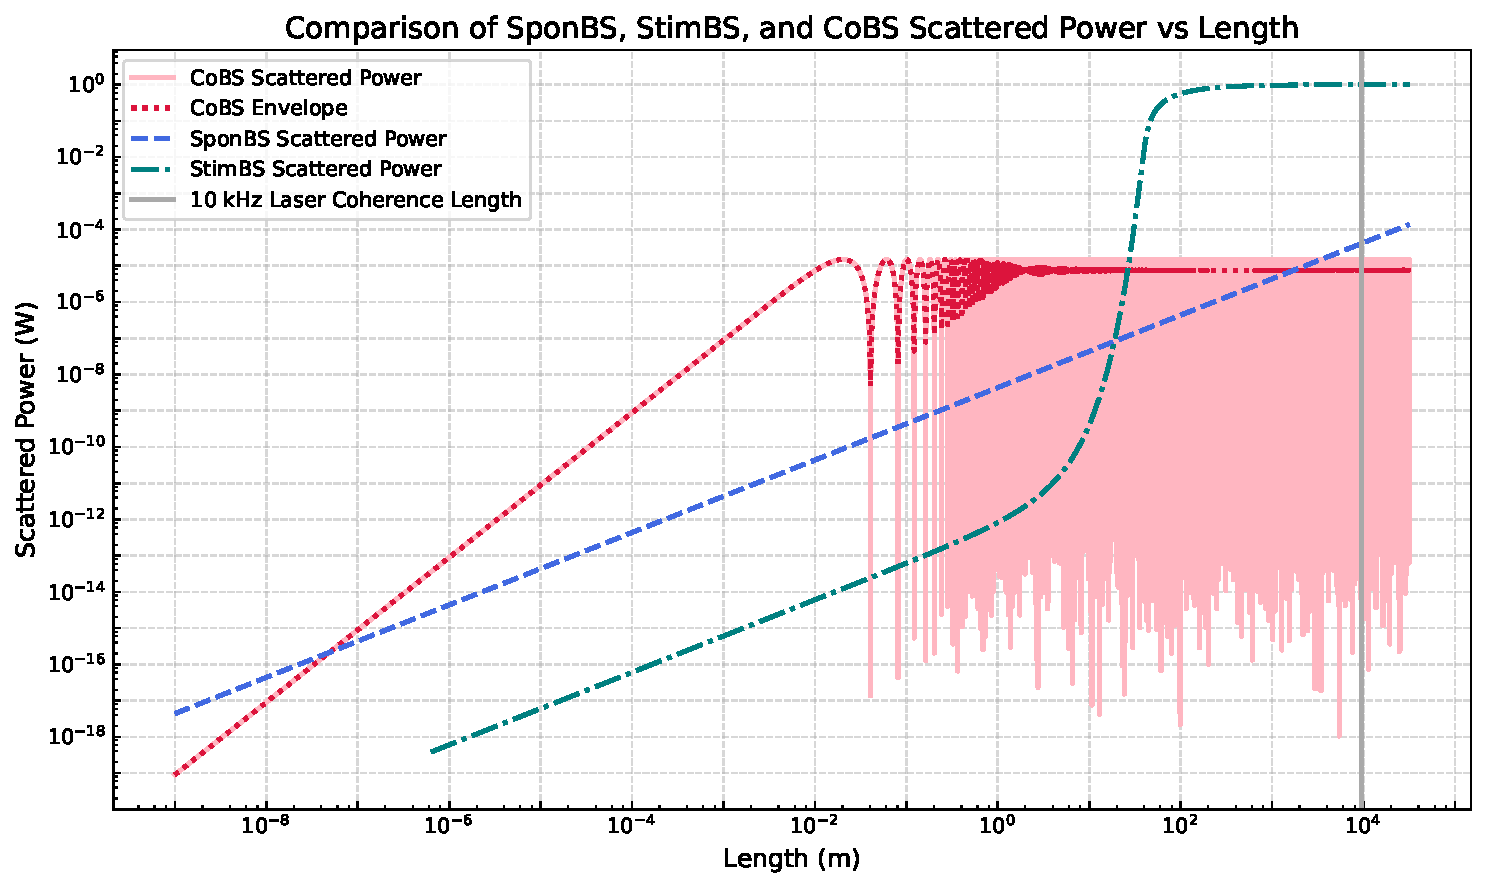
\includegraphics[width=\textwidth]{SponBSvsStimBSvsCoBS.pdf}
\caption{Comparison of scattered power from a spontaneous Brillouin scattering process and our coherently stimulated Brillouin spectrometer.}
\label{fig:SponBSvsStimBSvsCoBS}
\end{figure}

Fig.~\ref{fig:SponBSvsStimBSvsCoBS} shows the advantage that our coherently stimulated Brillouin spectrometer offers compared to the traditional Brillouin processes for the example medium of UHNA3 fiber. For lengths up to aboutces \SI{50}{\meter} and down to as low as \SI{100}{\nano\meter}, the coherently stimulated process employed by our instrument offers superior scattered power, with the relative advantage peaking for a length just over \SI{1}{\centi\meter}. At this length, the gain factor \(G\) places the traditional process within the low-gain (spontaneous) regime, and thus the scattered power generated is only on the order of tens of \si{\pico\watt}. In contrast, the scattered power offered by our instrument for the same system and identical powers is on the order of tens of \si{\micro\watt}, exceeding that of the spontenous process by a factor of \(10^6\). This is, of course, the most ideal case for this system, however it can be seen from Fig.~\ref{fig:SponBSvsStimBSvsCoBS} that the coherently stimulated process offers orders of magnitude more scattered power than either traditional process through a wide range of lengths.


% The scattered power produced by our instrument is approximately $1.07 \, \mu W$, which is readily detectable with standard photodetectors. This comparison demonstrates that, under identical experimental conditions, our instrument produces a significantly higher scattered power than SBS in a short fiber length. This is because SBS relies on amplifying a weak initial Stokes wave over a short interaction length, but the low gain parameter and phonon dissipation prevent significant amplification, resulting in an undetectable scattered power. Our technique, however, utilizes strong input waves and coherent interactions, leading to a measurable scattered signal even in short length media. Therefore, our instrument offers a significant advantage over SBS for generating detectable scattered signals with low Brillouin gain or small interaction length.

\newpage

\section{Observance of Fano-Resonant Asymmetries at Small Signals}
\label{Appendix:Fano}

In the main text (\textit{Fano-Resonant Asymmetries at Small Signals} in Sec.~\ref{Results}), we discussed how Fano-type interference can distort Brillouin line shapes in situations where the resonant Brillouin amplitude becomes comparable to the background continuum. We focus here on two experiments (A and B) that reveal these Fano asymmetries especially clearly. Experiment~A is a measurement series using the same \SI{1}{\centi\meter} UHNA3 fiber referenced in the main discussion, for which the main text showed only the fitted amplitudes (Fig.~\ref{fig:Phase-Match}). Here we show the full spectra, illustrating the emergence of asymmetries at lower amplitude conditions. Experiment~B is a distinct measurement involving a short (\(\sim\)\SI{1}{\milli\meter}) bulk liquid sample of carbon disulfide (\ce{CS2}) that we briefly mentioned in Sec.~\ref{Results:Fano-Resonant Asymmetries at Small Signals} but did not detail. This experiment was performed specifically to further probe the unexpected Fano-like distortions observed in Experiment~A. In each case, we outline the experimental setup, present the spectra, and highlight the appearance of Fano resonances. These observations corroborate the theoretical discussion of Fano line shapes (Sec.~\ref{Results:Fano-Resonant Asymmetries at Small Signals}) and provide insight into when and why they are most prominent.

\subsection{Experiment A: Extended 1\,cm UHNA3 Fiber Spectra}
\label{Appendix:Fano:Experiment A}

In the main text, we introduced a phase-matching experiment on \SI{1}{\centi\meter} of UHNA3 fiber in which the pump--probe detuning was varied from \SI{5}{\giga\hertz} to \SI{42}{\giga\hertz} in \SI{0.5}{\giga\hertz} increments. There, we reported only the resulting peak amplitudes, showing how they follow a \(\mathrm{sinc^{2}}\) dependence on detuning (Fig.~\ref{fig:Phase-Match} in the main text). However, each measurement in that scan also yields a full Brillouin spectrum—75 in total. Here, we present all 75 spectra to illustrate how the line shape transitions from nearly Lorentzian (when the Brillouin peak amplitude greatly exceeds the background continuum) to distinctly Fano-like (when the two amplitudes are comparable). We used the same setup and procedure described in \textit{Phase Matching Characterization} in Sec.~\ref{Results} of the main text. As the pump-probe detuning increases, the phase-matching term \(\mathrm{sinc^{2}(\Delta kL/2)}\) oscillates through peaks and troughs, causing the Brillouin peak amplitude to rise and fall. When the amplitude is sufficiently large, the Brillouin mode dominates the continuum and the spectrum appears nearly Lorentzian; when it drops to the order of the background amplitude, strong interference skews the line shape into a Fano-like profile.

\begin{figure}[h]
\centering
\includegraphics[height=0.95\textheight]{JoyDivisionCABSUHNA3.pdf}
\caption{Stacked Brillouin spectra showing Fano‐type line‐shape distortions at small signals in a \SI{1}{\centi\meter} UHNA3 fiber. Each trace corresponds to a different pump–probe detuning, revealing the discrete Brillouin resonance (near \SI{9.17}{\giga\hertz}) interfering with a broad continuum background. The resulting asymmetries highlight the characteristic Fano-resonant behavior under low signal conditions.}
\label{fig:Joy Division UHNA3}
\end{figure}

Figure~\ref{fig:Joy Division UHNA3} highlights the progressive shift from Lorentzian to asymmetric line shapes. Near \SI{5}{\giga\hertz} detuning (top spectra), the resonant amplitude is large relative to the background, giving a classic Lorentzian peak (\(q\to\infty\)) at \(\sim\)\SI{9.17}{\giga\hertz}. By contrast, at detunings between \(\sim\)15-\SI{20}{\giga\hertz} (where the \(\mathrm{sinc^{2}}\) factor is near a local minimum), the peak amplitude falls to roughly the same level as the continuum, and Fano interference is observed. Interestingly, as the detuning is increased further, and the amplitude rises again on a subsequent \(\mathrm{sinc^{2}}\) “lobe,”, the spectra partly recover a Lorentzian shape. This cyclical behavior persists, with each local maximum yielding a near-Lorentzian profile and each local minimum reintroducing a strong Fano distortion. These observations confirm the relationship between Brillouin peak amplitude and continuum interference described in \textit{Fano-Resonant Asymmetries at Small Signals} in Sec.~\ref{Results}. When the Brillouin amplitude significantly exceeds the background, the discrete phonon resonance dominates, resulting in little or no asymmetry (\(q\to\pm\infty\)). Once the two amplitudes become comparable, Fano interference skews the line shape, shifting the apparent peak frequency slightly and altering the slope on one side of the resonance. Analyzing selected spectra with both Lorentzian and Fano fits indicates that ignoring these distortions can lead to up to a 5–10\% misestimation of peak amplitude in the “trough” (low-amplitude) sets. This underscores the importance of employing a Fano model—particularly in small-signal measurements where the Brillouin peak may not tower over the background.

\subsection{Experiment B: 1\,mm \ce{CS2} Spectra and Fano Distortions}
\label{Appendix:Fano:Experiment B}

We now turn to measurements on a \SI{1}{\milli\meter}-thick cell of \ce{CS2} in a free-space geometry, complementing the \SI{1}{\centi\meter} UHNA3 fiber results (Experiment~A). Both experiments used comparable sub-Watt optical powers (on the order of \(\sim\)60–\SI{70}{\milli\watt} pump, \(\sim\)25–\SI{30}{\milli\watt} Stokes, and \(\sim\)40–\SI{50}{\milli\watt} probe). However, unlike Experiment~A—which probed a \SI{1}{\centi\meter} fiber with \SI{0.5}{\giga\hertz} detuning increments from \SI{5}{\giga\hertz} to \SI{42}{\giga\hertz}—here the detuning is stepped in \SI{0.25}{\giga\hertz} increments between \SI{10}{\giga\hertz} and \SI{14}{\giga\hertz}. Because the \ce{CS2} sample is an order of magnitude shorter (\SI{1}{\milli\meter} vs.\ \SI{1}{\centi\meter}), its phase-matching bandwidth (\(\mathrm{sinc}^{2}\) profile) is roughly ten times wider, making these \SI{0.25}{\giga\hertz} steps effectively twenty times finer than the \SI{0.5}{\giga\hertz} steps used in the fiber experiment. This reduced range of detunings within a broader \(\mathrm{sinc^2}\) profile produce measured peaks all of similar amplitude to one another, as opposed to the dynamic evolution of peaks in the \SI{1}{\centi\meter} UHNA3 fiber data.

Figure~\ref{fig:Joy Division CS2} shows all 17 spectra obtained at detuning increments of \SI{0.25}{\giga\hertz}, presented in order of increasing detuning from top spectrum to bottom spectrum. Each trace is offset vertically for clarity, with the topmost spectrum corresponding to \SI{10}{\giga\hertz} and the bottom spectrum corresponding to \SI{14}{\giga\hertz} detuning of the pump and the probe. A change in the detuning of the pump and probe via adjustment of the probe laser wavelength produces a change in phase of the resonant Brillouin signal. This changing resonant Brillouin phase relative to the background continuum produces spectra with different Fano-resonant distortions corresponding to specific values of the Fano parameter \(q\), as discussed in \textit{Fano-Resonant Asymmetries at Small Signals} (Sec.~\ref{Results}). Fano-asymmetries are seen in nearly every spectrum of this liquid experiment, indicating that the background continuum is competing strongly with the Brillouin amplitude in all measurements despite the advantage of broadened phase matching bandwidth. This lower Brillouin amplitude is owing to the order of magnitude shorter sample length and roughly two orders of magnitude larger effective area in our free-space configuration compared to that of the UHNA3 fiber in Experiment~A.

\begin{figure}[t]
  \centering
  \includegraphics[width=0.7\textwidth]{JoyDivisionCABSCS2.pdf}
  \caption{All measured Brillouin spectra for \SI{1}{\milli\meter}\,\ce{CS2} at detuning steps of \SI{0.25}{\giga\hertz} from \SI{10}{\giga\hertz} (top spectrum) to \SI{14}{\giga\hertz} (bottom spectrum). Each trace is offset for clarity.}
  \label{fig:Joy Division CS2}
\end{figure}

To illustrate how the Fano asymmetry parameter \(q\) can be positive or negative, we focus on two particular detunings that yielded notably skewed line shapes: \SI{10.75}{\giga\hertz} and \SI{13.5}{\giga\hertz}. Figure~\ref{fig:CS2FanoCompare} compares the spectra for these two detunings, overlaid with both a Lorentzian fit (dashed lines) and a Fano fit (solid lines). The insets show residuals (data minus fit). The measured peak of the \SI{13}{\giga\hertz} spectrum (Fig.~\ref{fig:CS2FanoCompare}b) exhibits a sharper rise on the lower-frequency side and a gentler roll-off on the higher-frequency side, indicative of \(q>0\), whereas that of the \SI{13.75}{\giga\hertz} spectrum is skewed in the opposite sense,
featuring a sharper high-frequency side and a softer low-frequency slope, suggesting \(q<0\). Clearly, the Fano model captures the asymmetric tails better than a simple Lorentzian, especially around the half-maximum slopes.

Notably, in the negative-\(q\) case (\SI{13.75}{\giga\hertz}), the line’s peak amplitude appears slightly higher than what would be inferred from a Lorentzian fit—sometimes referred to as a “peak boost.” As discussed in \textit{Fano-Resonant Asymmetries at Small Signals} (Sec.~\ref{Results}), this can be beneficial for detecting weaker signals, provided the background is not too noisy, and in principle, one could choose a phase relationship that maximizes this constructive interference near resonance. Conversely, a positive-\(q\) scenario can suppress or broaden the peak on one side, which may be less desirable for line-shape analysis but could be exploited if one aims to shape the response profile in a particular way.

\begin{figure}[h]
  \centering
  \begin{subfigure}{0.45\textwidth}
    \centering
    % \includegraphics[width=\textwidth]{CS2FanoCompare-13GHz.pdf} % Replace with actual file name
    \caption{Representative spectrum at \SI{13}{\giga\hertz}, illustrating positive \(q\) asymmetry. Dashed lines are Lorentzian fits; solid lines are Fano fits. Residuals in the inset highlight the improved agreement of the Fano model.}
    \label{fig:CS2FanoCompare-13GHz}
  \end{subfigure}%
  \hfill
  \begin{subfigure}{0.45\textwidth}
    \centering
    % \includegraphics[width=\textwidth]{CS2FanoCompare-13.75GHz.pdf} % Replace with actual file name
    \caption{Representative spectrum at \SI{13.75}{\giga\hertz}, illustrating negative \(q\) asymmetry. Dashed lines are Lorentzian fits; solid lines are Fano fits. Residuals in the inset highlight the improved agreement of the Fano model.}
    \label{fig:CS2FanoCompare-13.75GHz}
  \end{subfigure}
  \caption{Comparison of representative spectra at (a) \SI{13}{\giga\hertz} and (b) \SI{13.75}{\giga\hertz}, showing the positive vs.\ negative \(q\) asymmetry in 1\,mm CS\textsubscript{2}. Residuals in the insets highlight the improved agreement of the Fano model over the Lorentzian model.}
  \label{fig:CS2FanoCompare}
\end{figure}

These \SI{1}{\milli\meter} \ce{CS2} data reinforce the conclusions from the UHNA3 fiber measurements, demonstrating that Fano-type asymmetries arise readily in small-signal regimes across diverse geometries (liquid cell vs.\ fiber). Moreover, we have explicitly identified positive- and negative-\(q\) cases, showing that interference can either boost or clip the Brillouin resonance peak, depending on the sign of \(q\) and the relative amplitude of the background continuum. As in Experiment~A, a Fano-fitting procedure is essential to extract accurate linewidths and center frequencies in these small-signal conditions.

\vspace{2em}

To better convey the cyclical evolution of the 75 measured UHNA3 spectra from Experiment~A, we have created an animated GIF that steps through each spectrum in ascending pump--probe detuning. This animation can be found in the Supplemental Material as a separate file. We also host the GIF (along with the raw data, measurement logs, and plotting scripts) in a public GitHub repository:
\[
\text{\url{https://github.com/HamletTheHamster/A-Coherently-Stimulated-Brillouin-Spectrometer}}
\]
Readers are encouraged to view it for a clear, dynamic perspective on how the line shape transitions between Lorentzian and Fano-distorted forms at different detunings.


\newpage

\section{Pump, Stokes, and Probe Contribute Equally}

Eq.~\ref{Eq:Theoretical Framework:Scattered Power} gives the somewhat unintuitive result that the powers of the Pump, Stokes, and Probe waves contribute equally to the resulting scattered power of the Signal and invites verification with a miniexperiment. Initially, this experiment was motivated by a practical consideration: determination of whether the placement of a high power amplifier on any specific line of the setup (Pump, Stokes, or Probe) would offer any advantage over another.

To test this, we conducted a controlled experiment with a 1 mm carbon disulfide (\ce{CS2}) sample. For each measurement, one of the three source powers (Pump, Stokes, or Probe) was systematically reduced by 75\% while holding the others constant and ensuring consistent experimental conditions across trials. Table~\ref{tab:PSPr-Contribute-Equally} shows the respective powers for each source during the three measurements, along with the multiplicative total contribution of the three powers for each measurement towards the generation of scattered power of the Signal.

\begin{table}[h]
  \centering
  \renewcommand{\arraystretch}{1.2}
  \begin{tabular}{|c|c|c|c|c|}
    \hline
    \textbf{Measurement} & \textbf{Pump Power (\si{\milli\watt})} & \textbf{Stokes Power (\si{\milli\watt})} & \textbf{Probe Power (\si{\milli\watt})} & \textbf{Total (\si{\milli\watt\cubed})} \\
    \hline
    Pump Lower & 19.190 & 32.210 & 54.560 & 3.372 \(\times 10^4\) \\
    Stokes Lower & 76.600 & 8.020 & 54.650 & 3.359 \(\times 10^4\) \\
    Probe Lower & 76.600 & 32.530 & 13.480 & 3.359 \(\times 10^4\) \\
    \hline
  \end{tabular}
    \caption{Power values for each source (Pump, Stokes, Probe) across the three measurements, with the multiplicative total power for each setup.}
    \label{tab:PSPr-Contribute-Equally}
\end{table}

Figure~\ref{fig:PSPr-Contribute-Equally} displays the average results from these three measurements, plotted with error bars representing one standard deviation of the mean. For increased certainty, Figure~\ref{fig:PSPr-Contribute-Equally-2sigma} presents the same data with error bars extended to two standard deviations, providing additional confidence in the reproducibility of the results. This experiment confirms that the scattered Signal power indeed depends equally on each of the three contributing wave powers, as expected from the theoretical framework. Consequently, boosting the power of any of the three sources affects the Signal power equally, allowing flexibility in pragmatic design across any of the three lines. Ultimately, this result reinforces the reliability of Equation \ref{Eq:Theoretical Framework:Scattered Power} for predicting Signal power across a range of power distributions within practical settings.

% \begin{figure}[h]
%   \centering
%   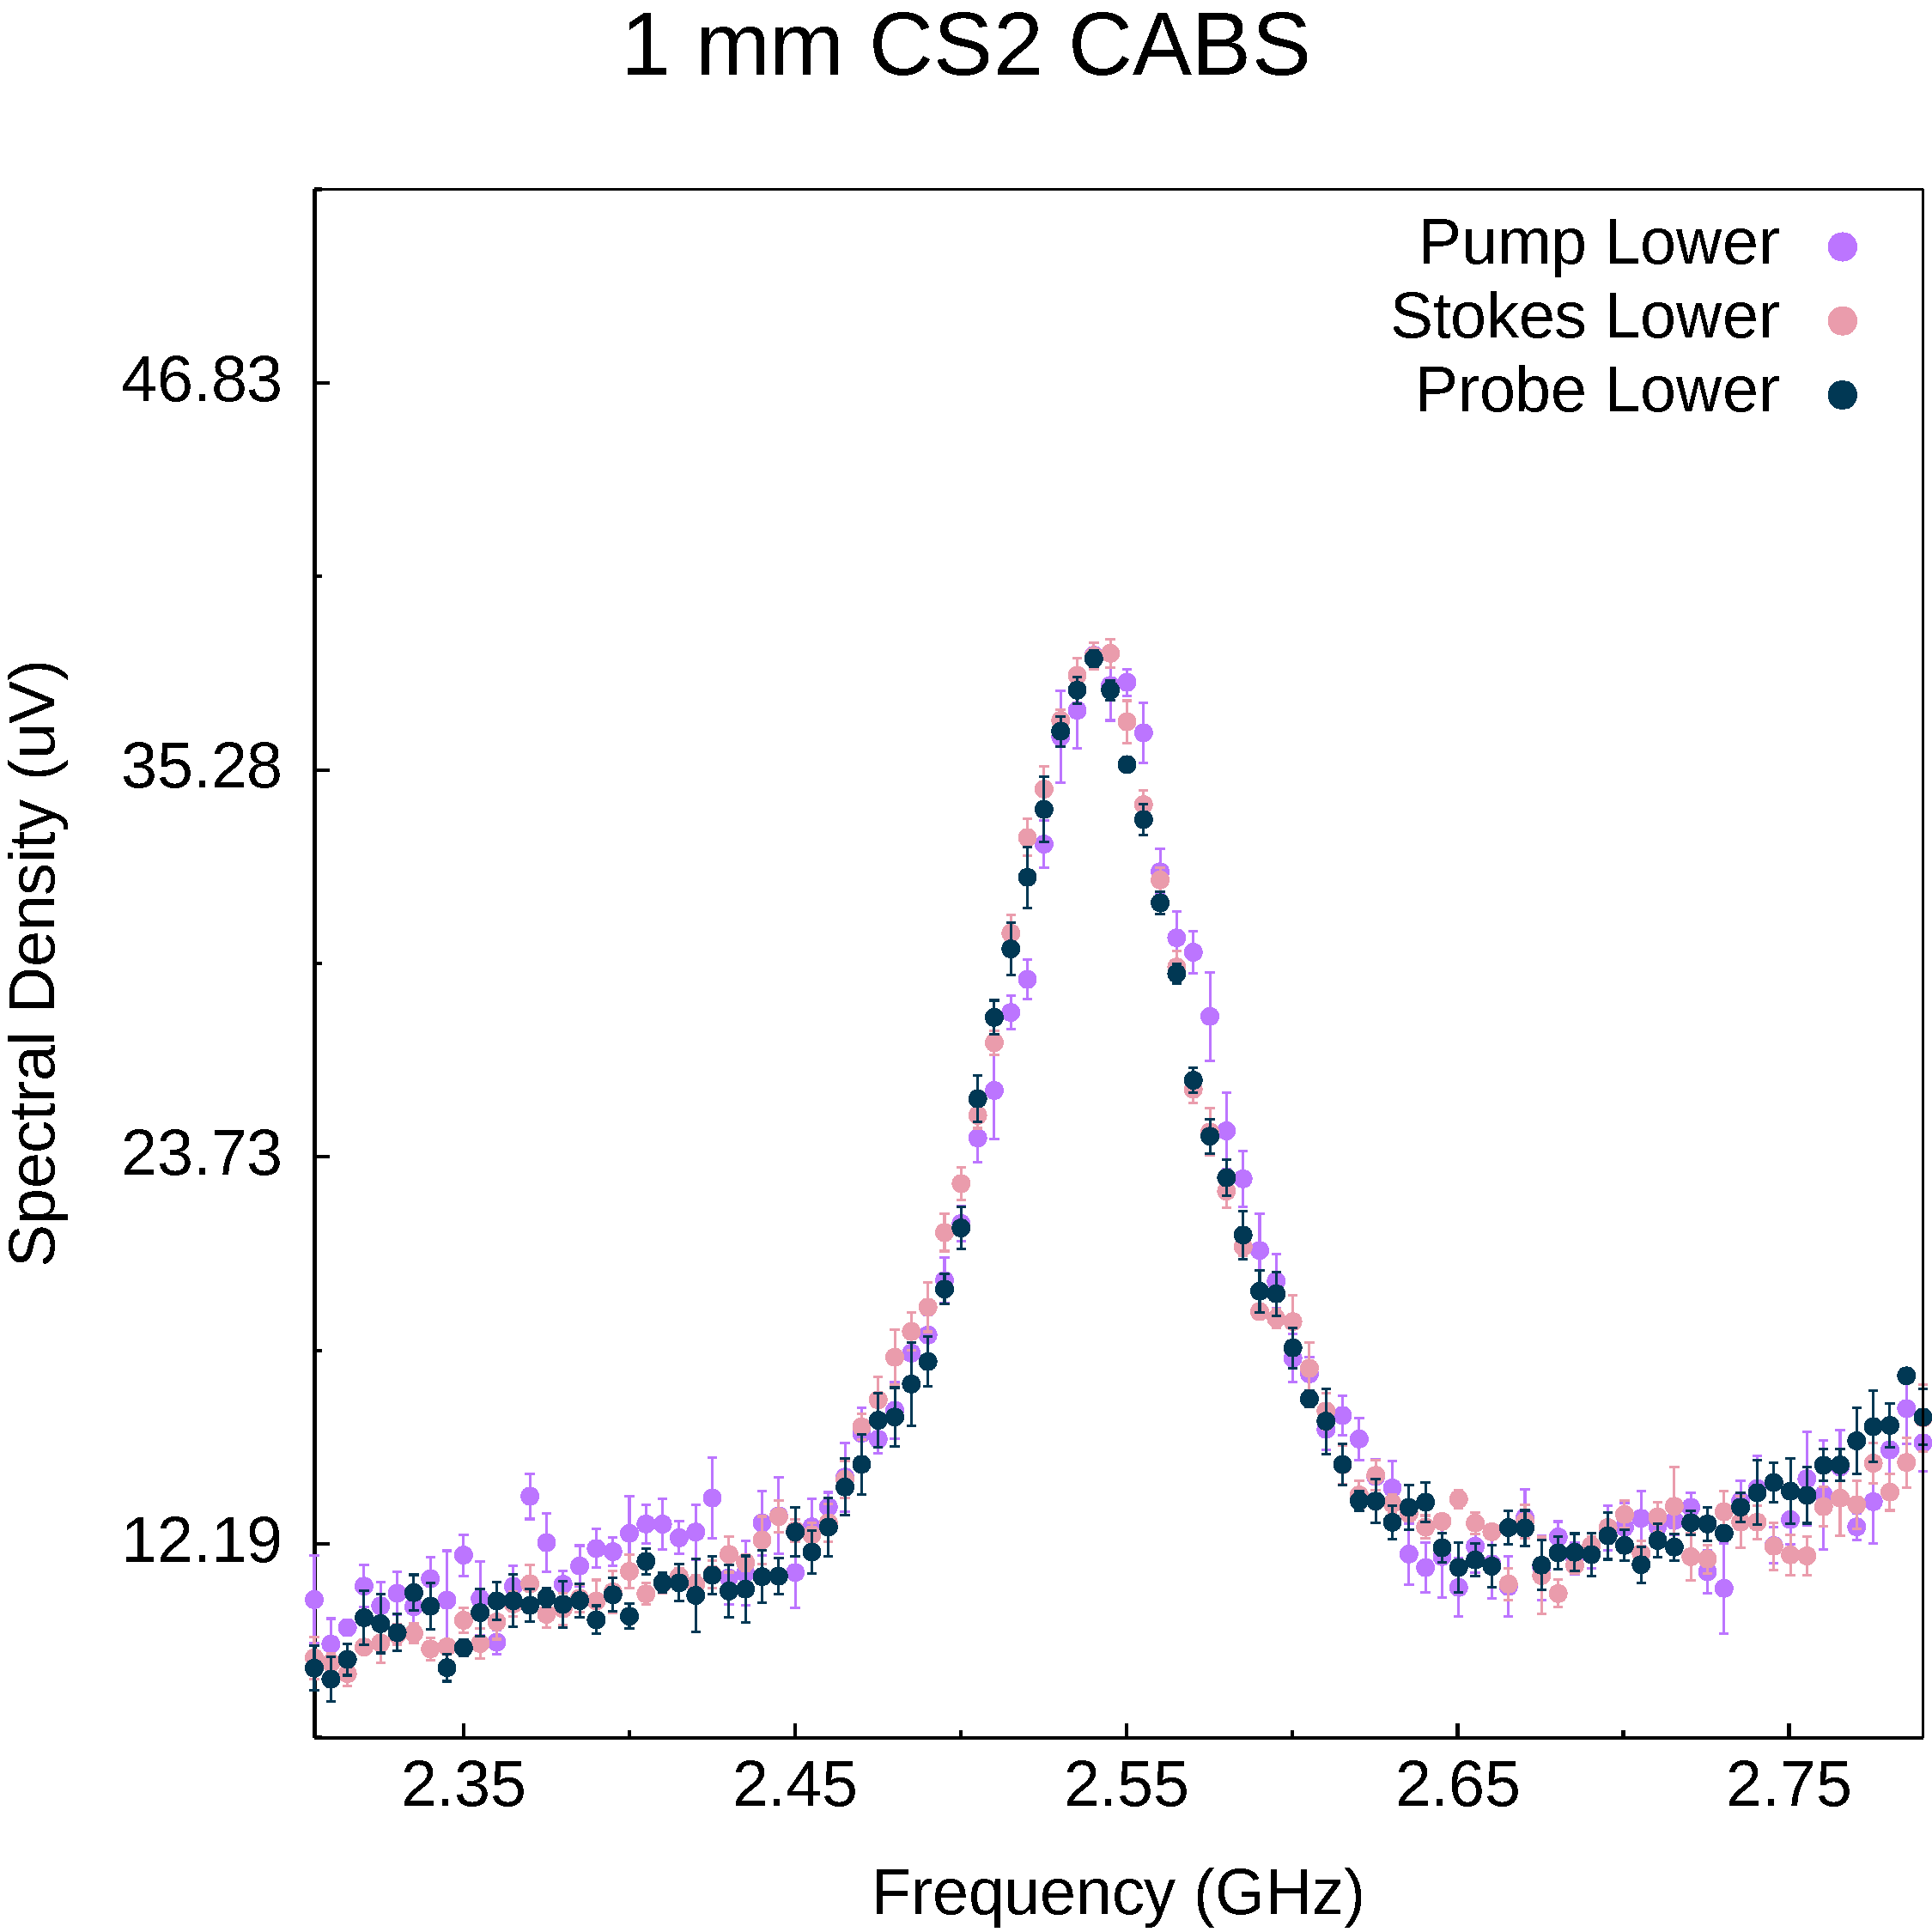
\includegraphics[width=.45\textwidth]{PSPr-Contribute-Equally.pdf}
%   \caption{Signal power contributions with error bars representing one standard deviation of the mean for each measurement.}
%   \label{fig:PSPr-Contribute-Equally}
% \end{figure}
%
% \begin{figure}[h]
%   \centering
%   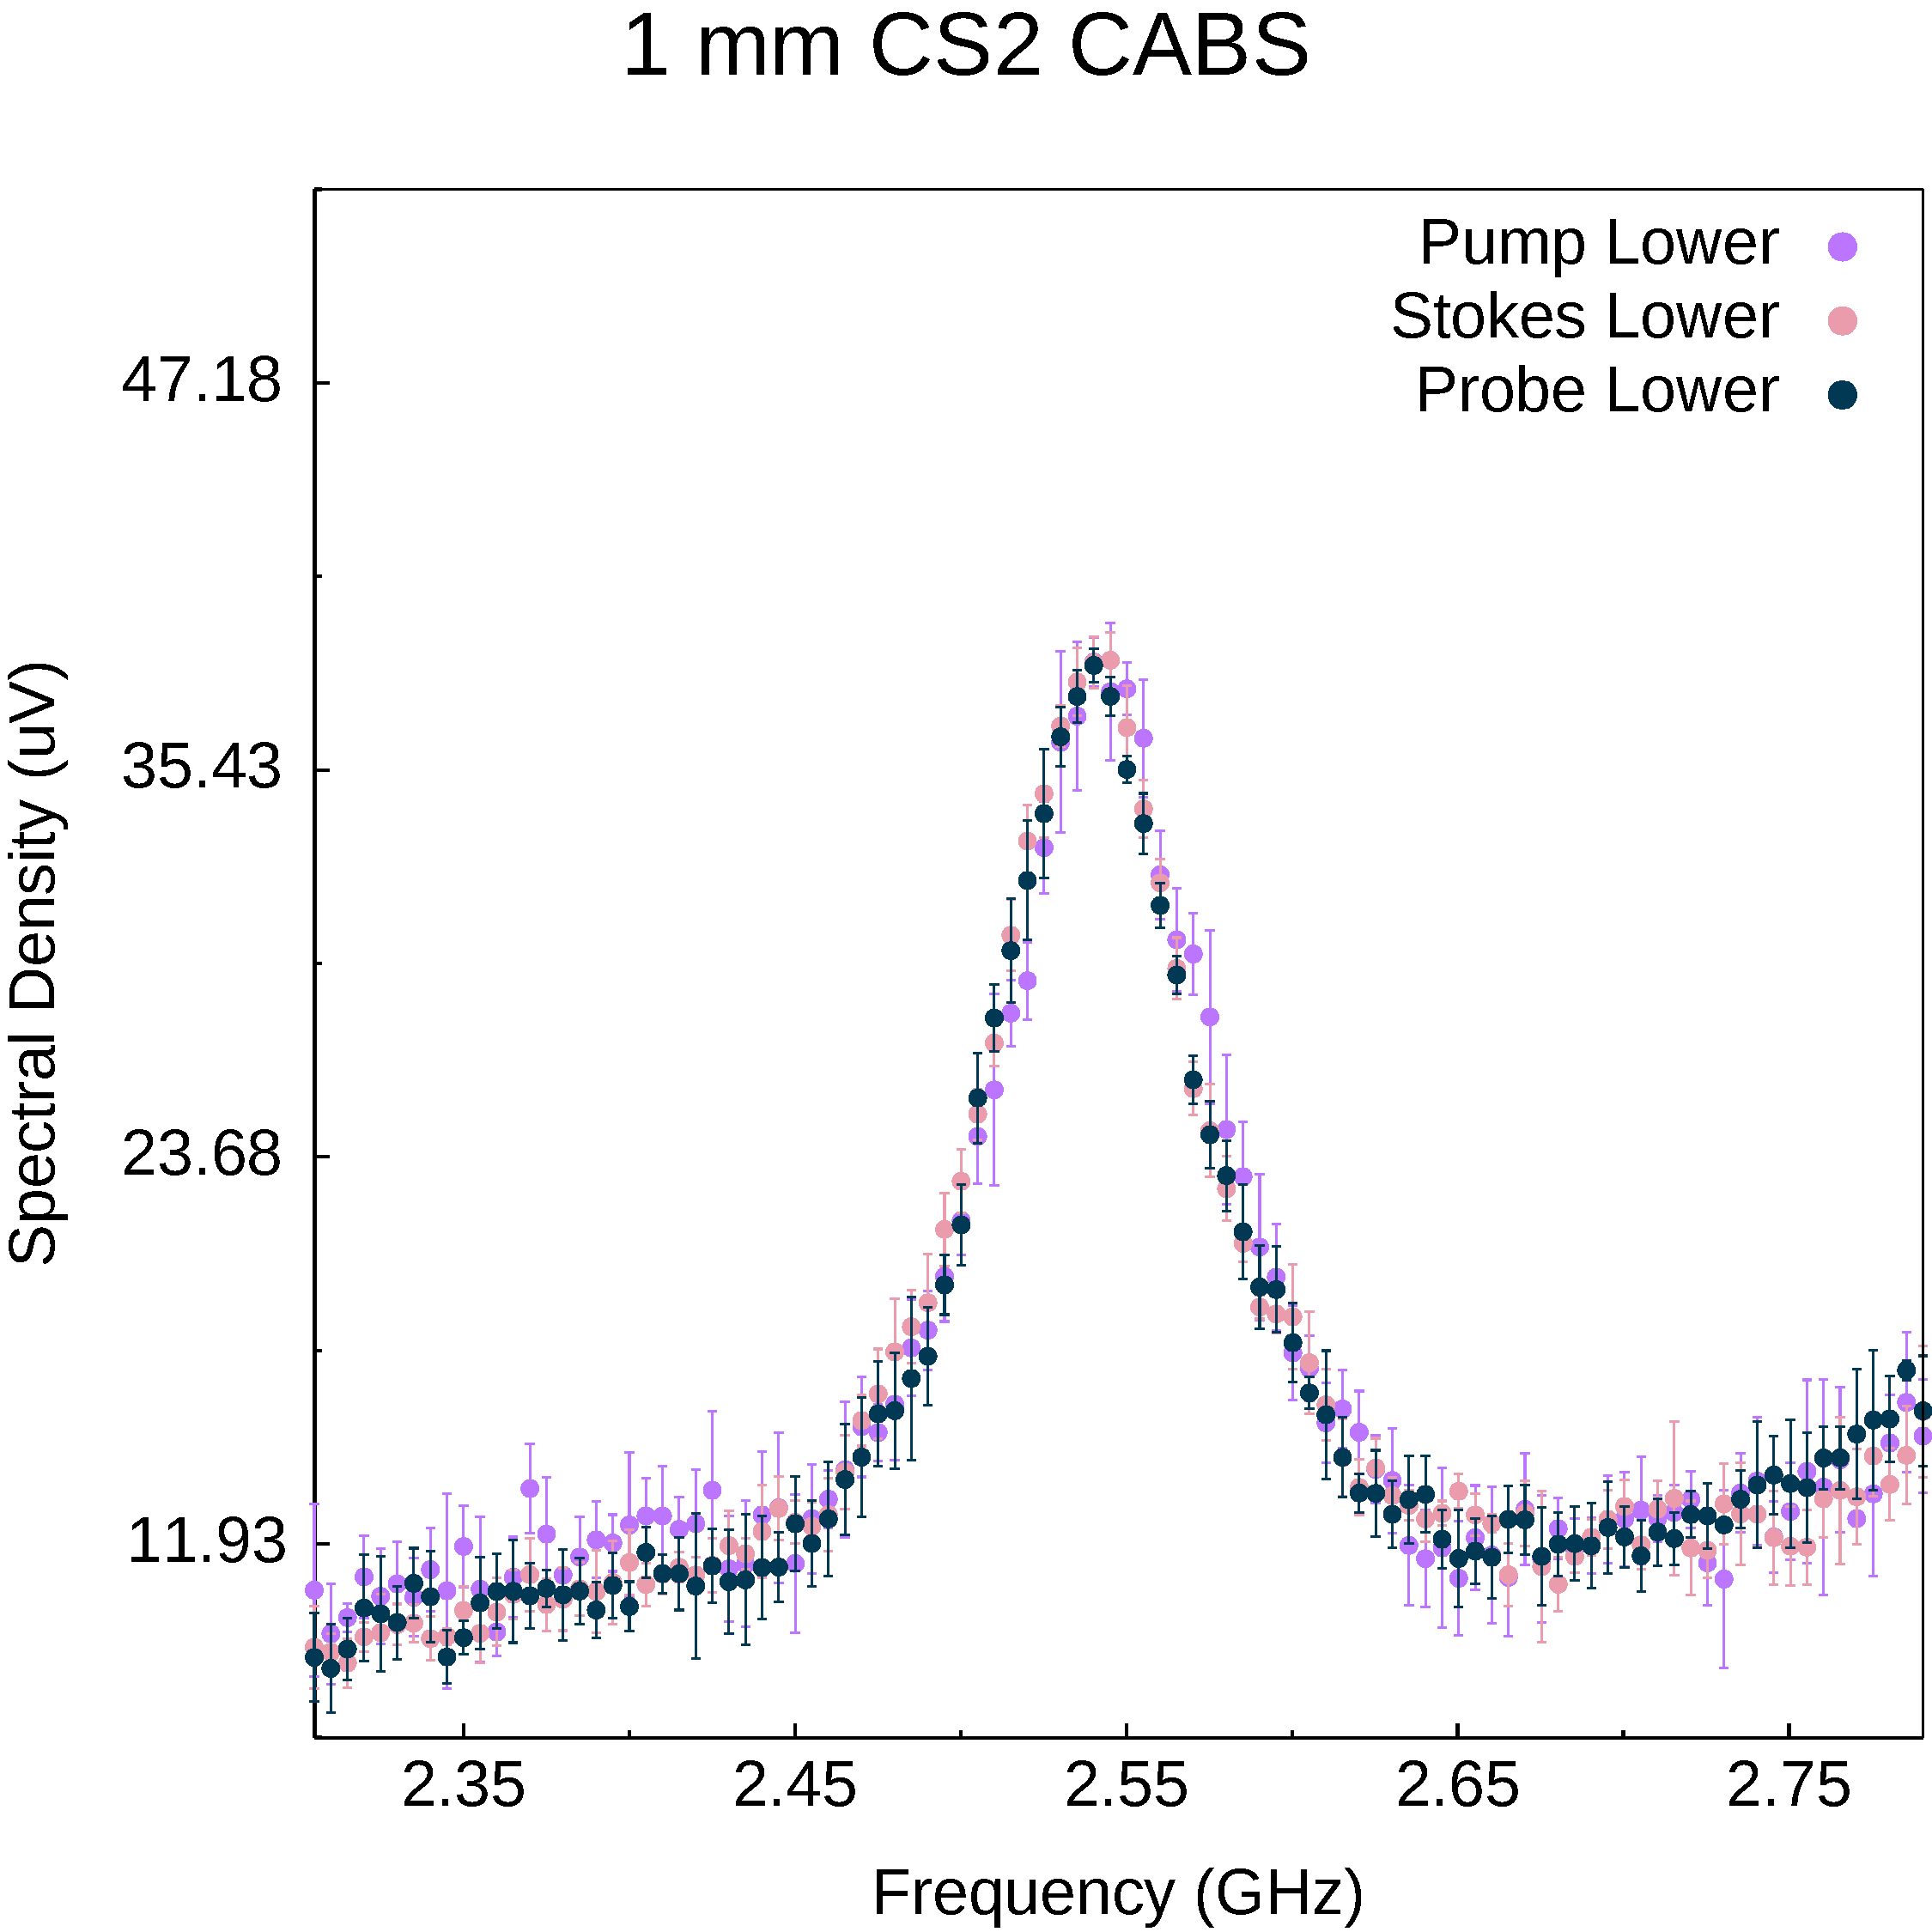
\includegraphics[width=.45\textwidth]{PSPr-Contribute-Equally-2sigma.pdf}
%   \caption{Signal power contributions with error bars extended to two standard deviations of the mean for each measurement.}
%   \label{fig:PSPr-Contribute-Equally-2sigma}
% \end{figure}

\begin{figure}[h]
  \centering
  \begin{subfigure}{0.45\textwidth}
    \centering
    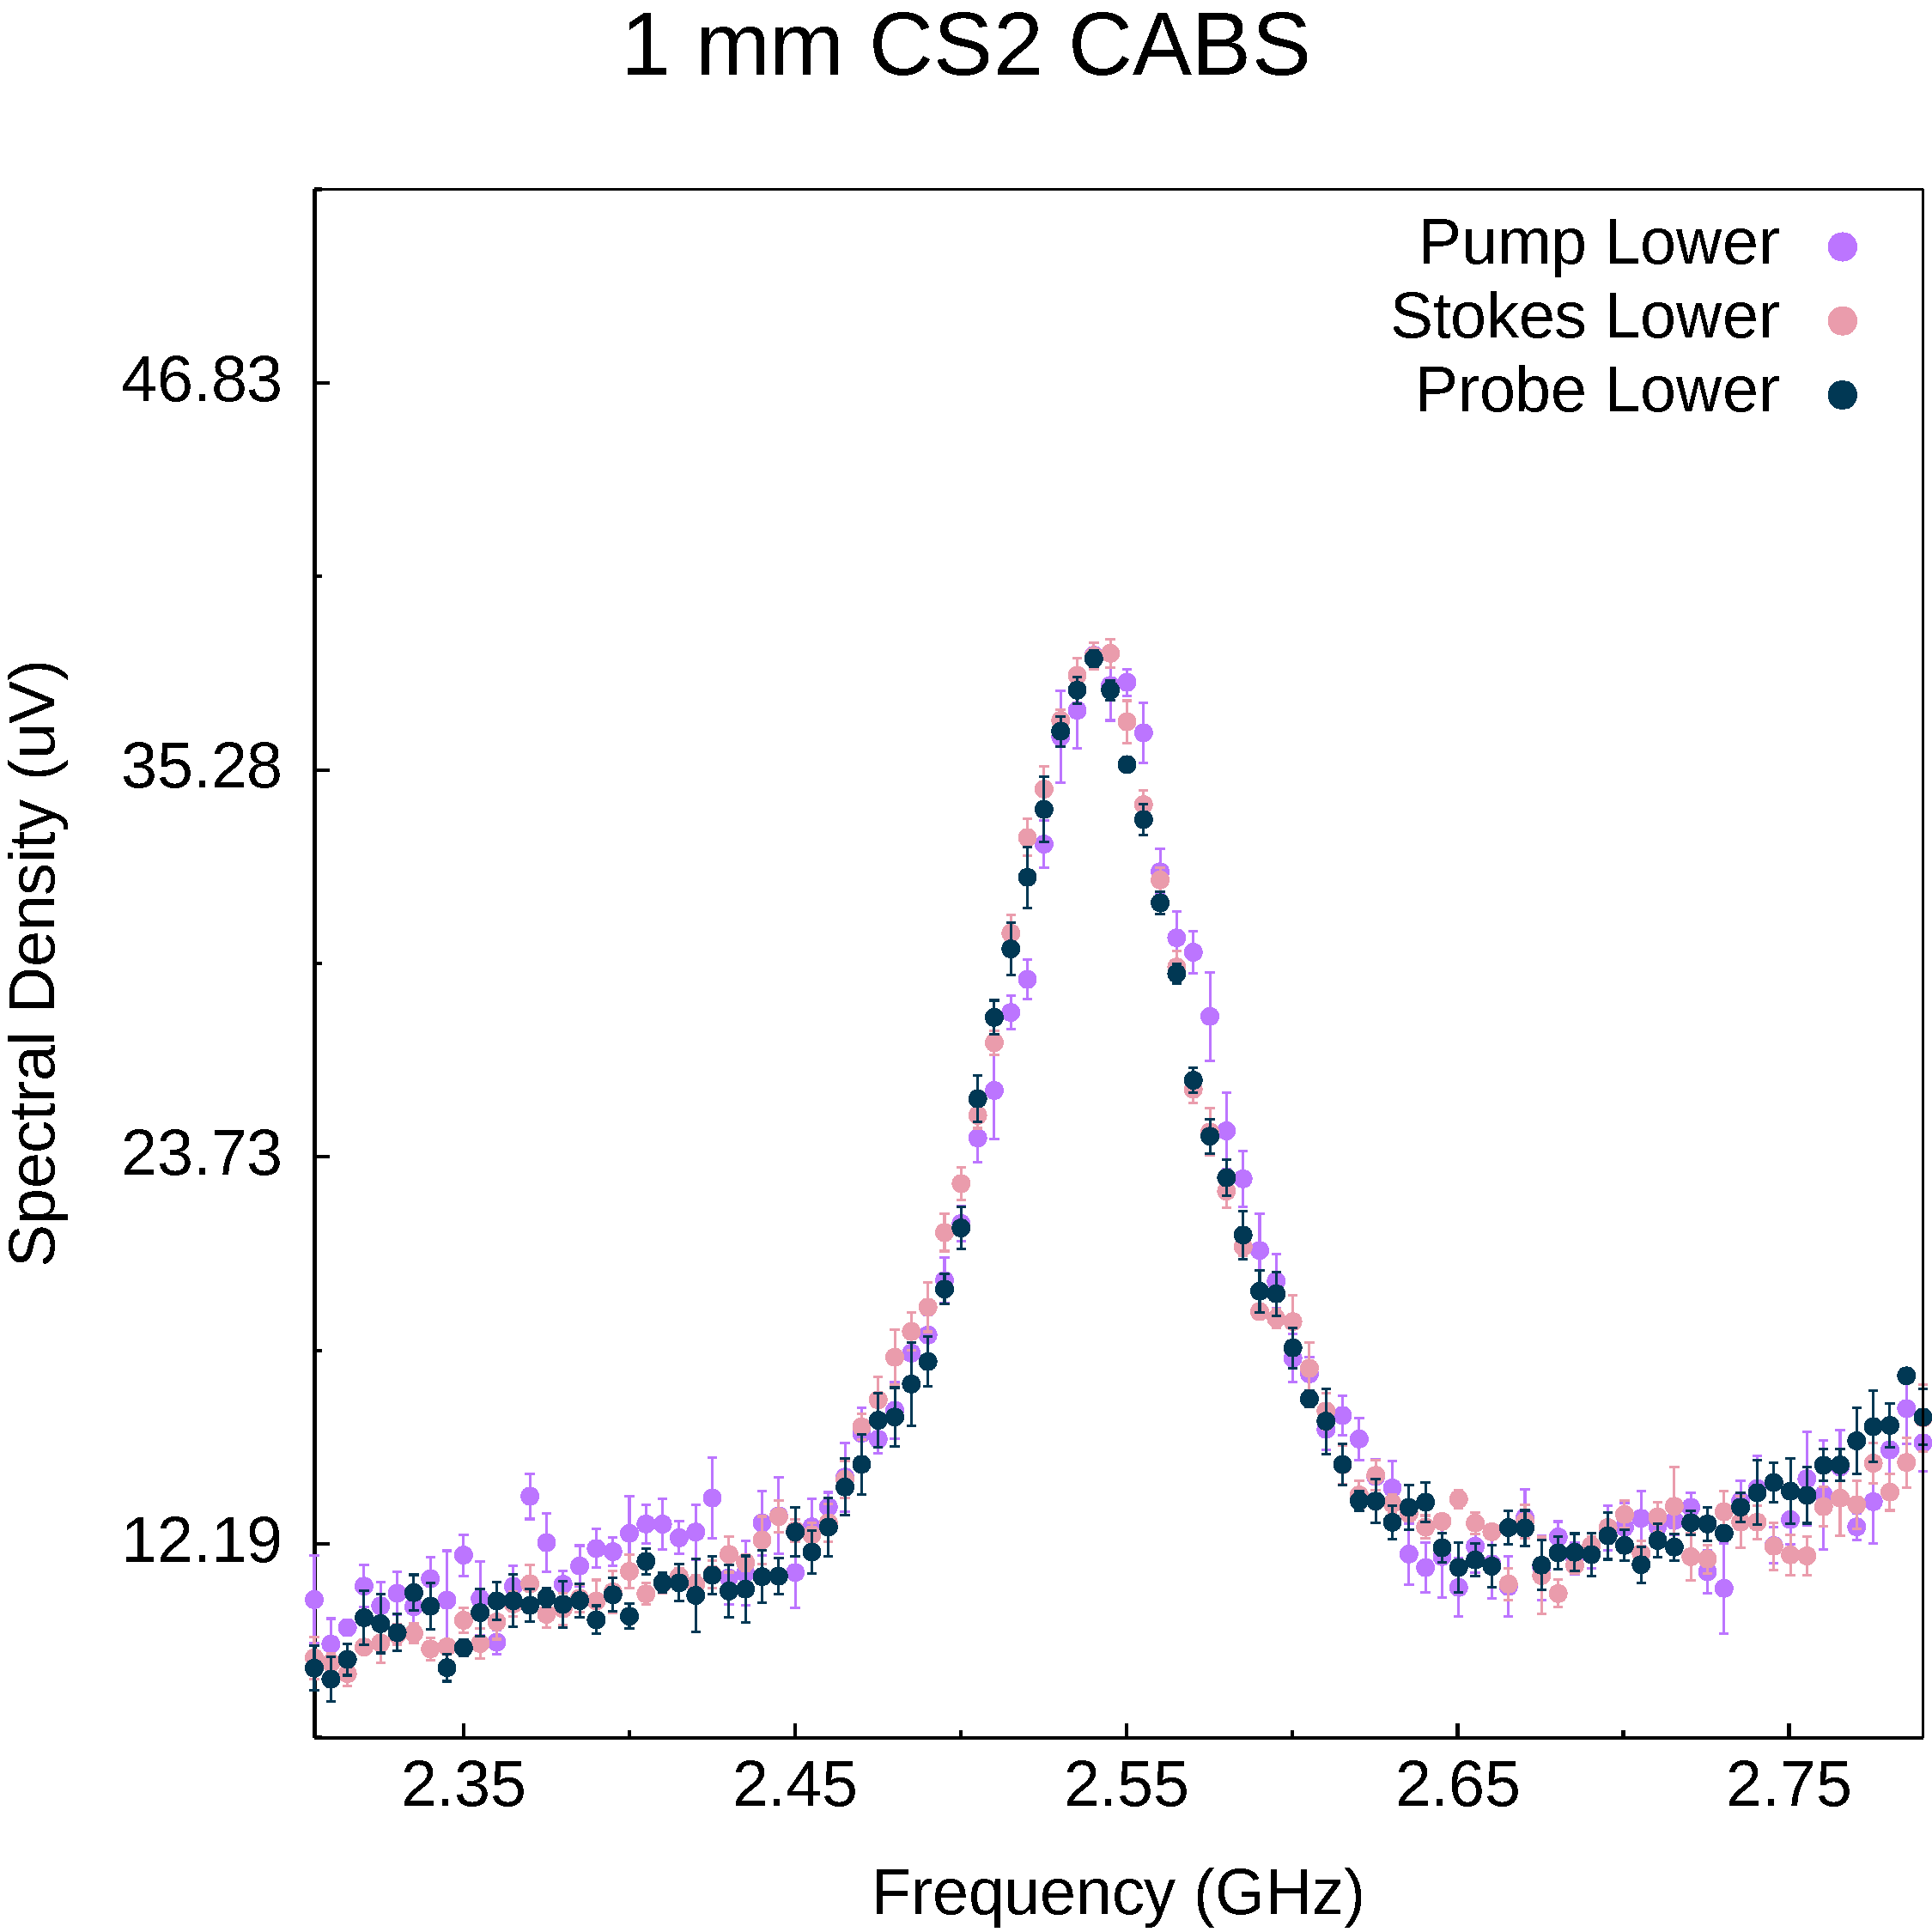
\includegraphics[width=\textwidth]{PSPr-Contribute-Equally.pdf}
    \caption{Signal power contributions with error bars representing one standard deviation of the mean for each measurement.}
    \label{fig:PSPr-Contribute-Equally}
  \end{subfigure}%
  \hfill
  \begin{subfigure}{0.45\textwidth}
    \centering
    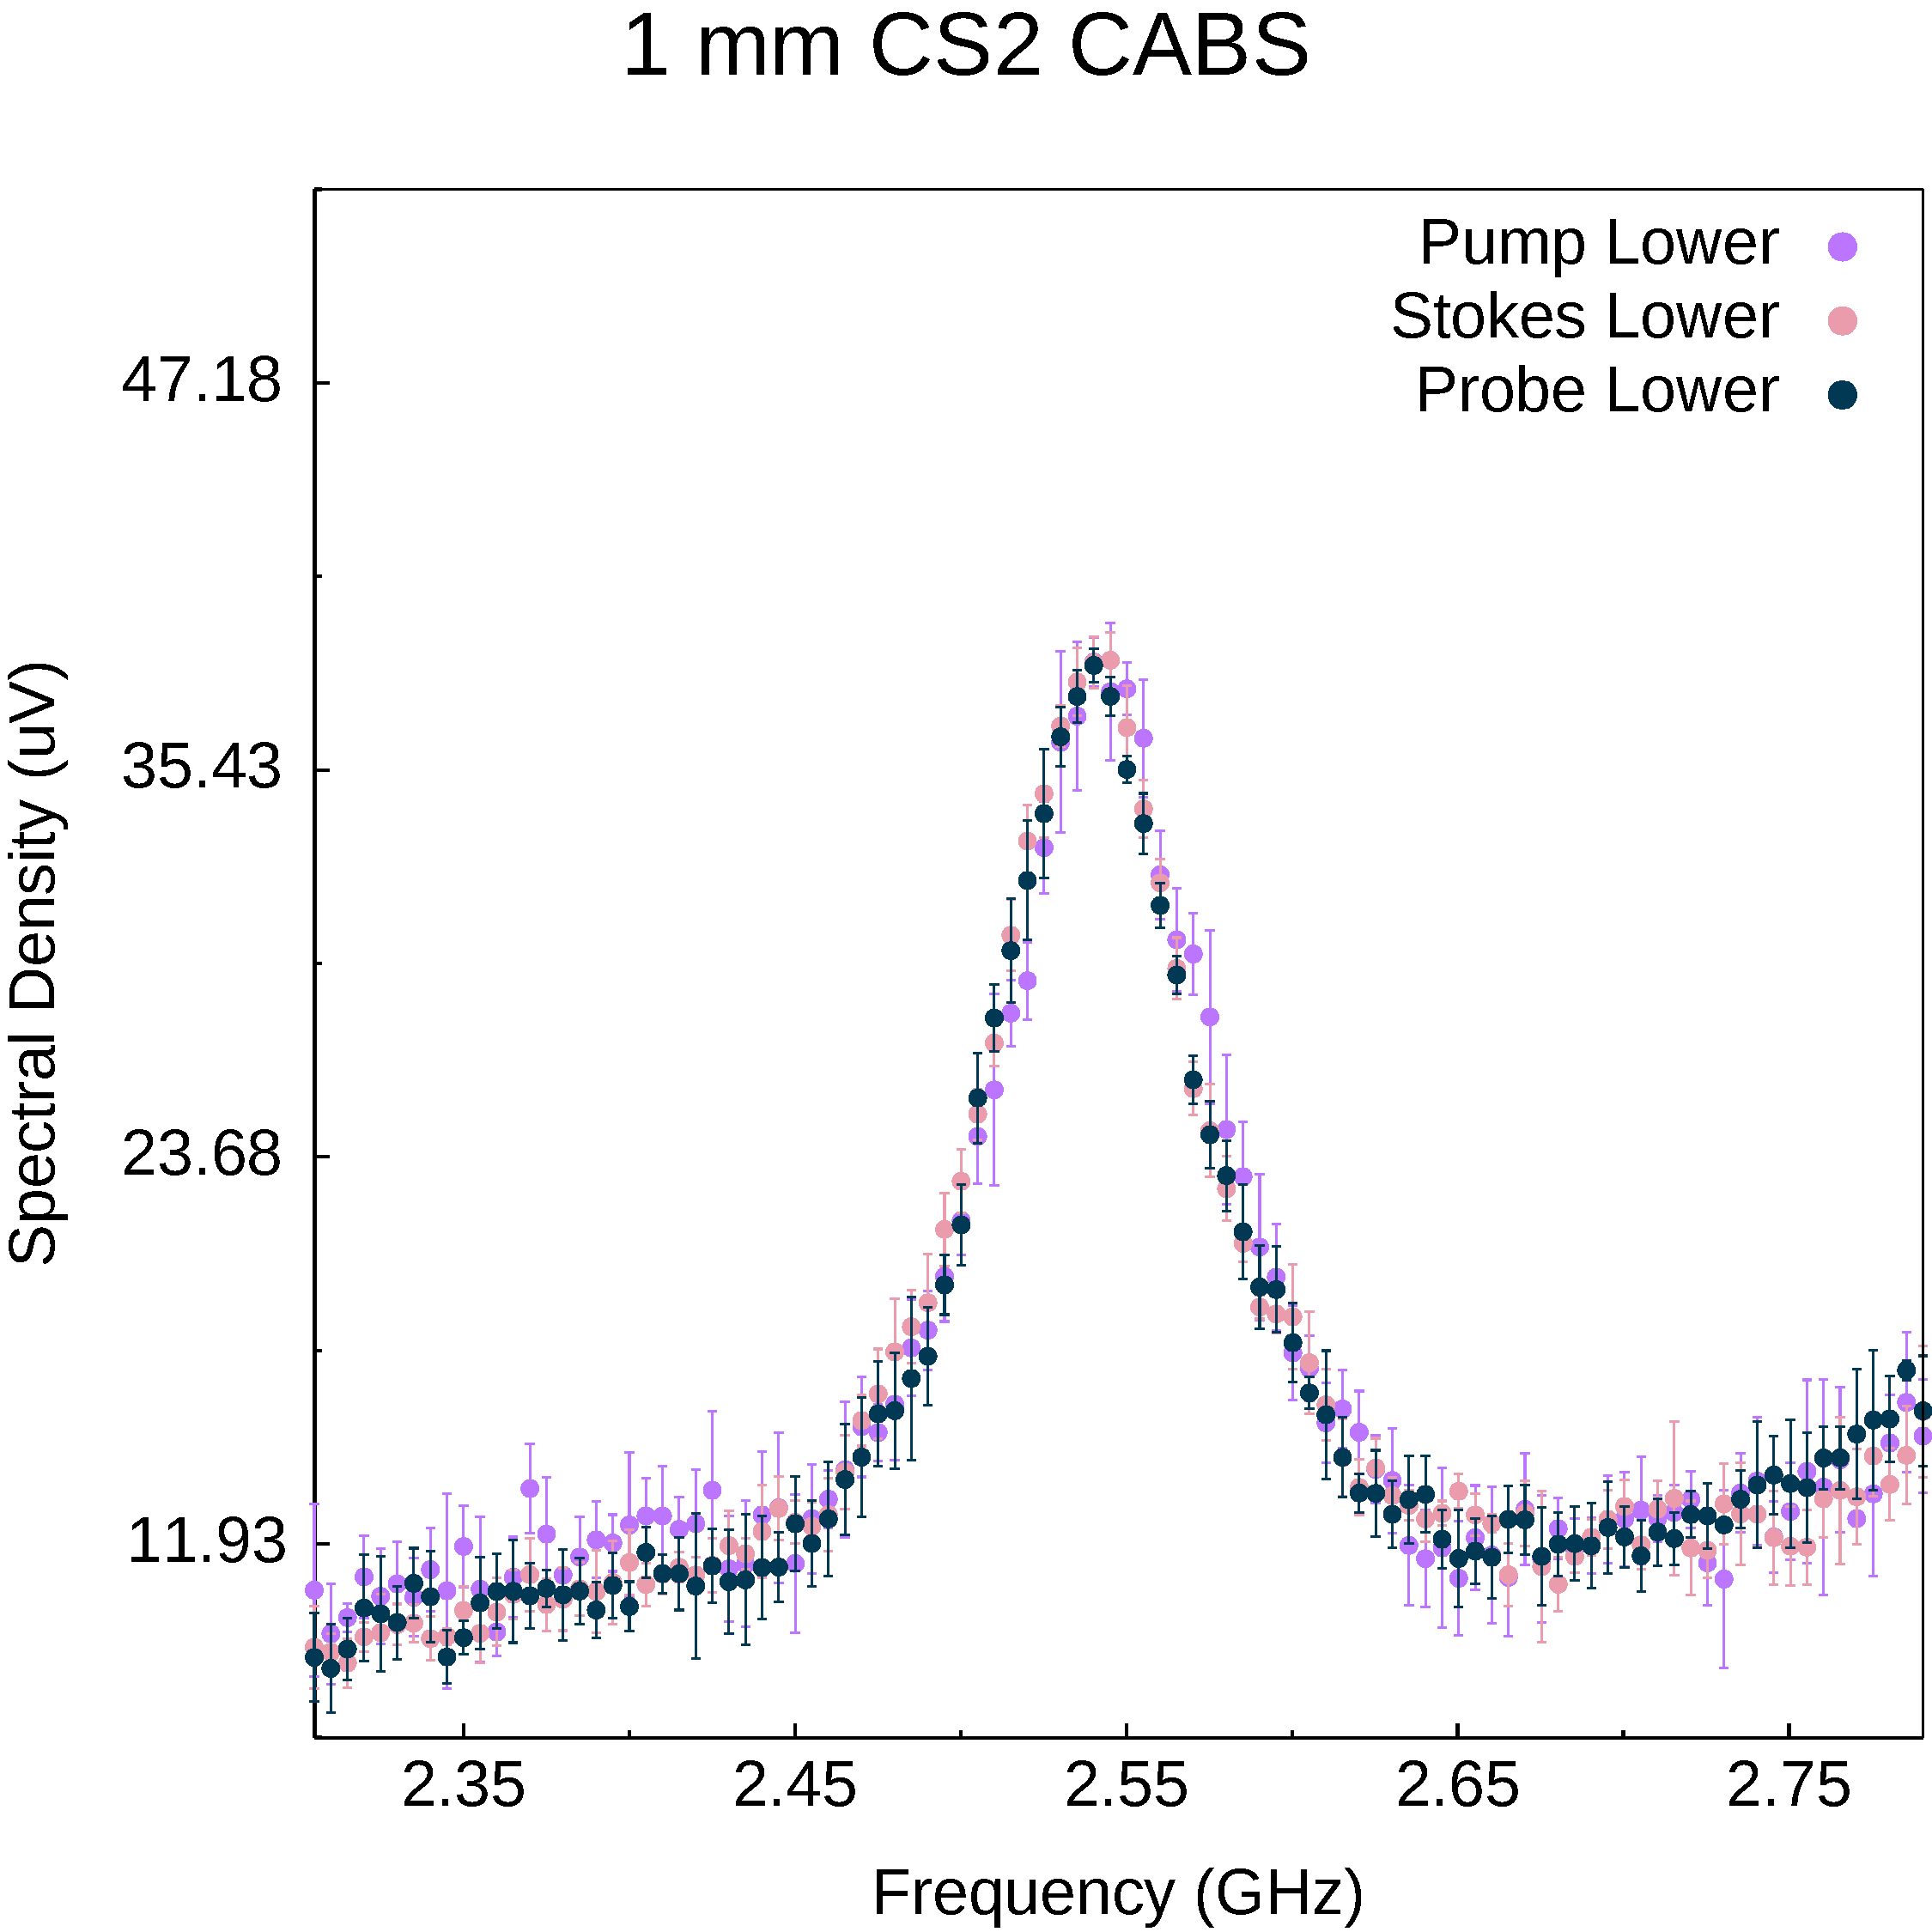
\includegraphics[width=\textwidth]{PSPr-Contribute-Equally-2sigma.pdf}
    \caption{Signal power contributions with error bars extended to two standard deviations of the mean for each measurement.}
    \label{fig:PSPr-Contribute-Equally-2sigma}
  \end{subfigure}
  \caption{Comparison of Signal power contributions with error bars representing one (a) and two (b) standard deviations of the mean for each measurement.}
  \label{fig:combined}
\end{figure}


\twocolumngrid

\bibliography{bibliography}% Produces the bibliography via BibTeX.

\end{document}
%
% ****** End of file apssamp.tex ******
